\chapter{Internet 协议}

\section{引言}
IP 是TCP/IP 协议族中的核心协议。所有 TCP、UDP、ICMP 和 IGMP 数据都通过IP 数
据报传输。IP 提供了一种尽力而为、无连接的数据报交付服务。“尽力而为”的含义是不保
证IP数据报能成功到达目的地。虽然IP 不是简单丢弃所有不必要流量,但它也不对自己尝
试交付的数据报提供保证。当某些错误发生时,例如一台路由器临时用尽缓冲区,IP 提供一
个简单的错误处理方法:丢弃一些数据(通常是最后到达的数据报)。任何可靠性必须由上
层(例如 TCP)提供。IPv4 和IPv6 都使用这种尽力而的基本交付模式。

“无连接”意味着IP 不维护网络单元(即路由器)中数据报相关的任何链接状态信息,
每个数据报独立于其他数据报来处理。这也意味着IP 数据报可不按顺序交付。如果一个源
主机向同一目的地发送两个连续的数据报(第一个为A,第二个为B),每个数据报可以独
立路由,通过不同路径,并且B可能在A之前到达。IP数据报也可能发生其他问题:它们
可能在传输过程中被复制,可能改变内容从而导致错误。此外,IP 之上的一些协议(通常是
TCP)需要处理这些潜在问题,以便应用提供无差错的交付。

本章我们首先看一下IPv4(见图5-1)和IPv6(见图5-2)头部中的字段,然后描述IP
如何转发。\href{https://www.rfc-editor.org/rfc/rfc0791}{[RFC0791]}是针对IPv4
的正式规范。描述 IPv6 的一系列
RFC从\href{https://www.rfc-editor.org/rfc/rfc2460}{[RFC2460]}开始。

图5-1 IPv4数据报。头部大小可变,4位的 IHL字段被限制为15个32位字(60字节)。一个典型的
IPv4 头部包含20字节(没有选项)。源地址和目的地址的长度32位。第二个32位字的大部分
用于 IPv4 分片功能。头部校验和有助于确保头部字段被正确发送到目的地,但不保护数据内容

IPv6 头部大小固定(40字节),并包含128位源地址和目的地址。下一个头部字段用于说明
IPv6头部之后其他扩展头部的存在和类型,它们形成一条包括特殊扩展或处理指令的头部链。
应用数据跟在这条头部链之后,通常紧跟着是一个传输层头部

\section{IPV4 头部和IPV6头部}
图5-1 显示了IPv4数据报格式。正常的IPv4 头部大小为20字节,除非存在选项(这种
情况很少见)。IPv6 头部长度是它的两倍,但没有任何选项。它可以有扩展头部,可提供类
似的功能,我们将在后面看到。在关于IP 头部和数据报的印象中,最高有效位在左侧且编
号为0,一个32位值的最低有效位在右侧且编号为31。

一个32位值的4字节按以下顺序传输:首先是0~7位,然后是8~15位,接着是
16 ~23位,最后是24~31位。这就是所谓的高位优先字节序,它是 TCP/IP 头部中所有二
进制整数在网络中传输时所需的字节顺序。它也被称为网络字节序。计算机的CPU 使用其
他格式存储二进制整数,例如大多数PC使用低位优先字节序,在传输时必须将头部值转换
为网络字节序,并在接收时再转换回来。

\subsection{IP 头部字段}
第一个字段(只有4位或半个字节)是版本字段。它包含IP 数据报的版本号:IPv4 为4,
IPv6 为6。IPv4头部和 IPv6头部除版本字段位置相同外再无其他是一样的。因此,这两个
协议不能直接互操作,主机或路由器必须分别处理IPv4或IPv6(或两者,称为双栈)。虽然
也提出并发展了其他IP版本,但只有版本4和6经常使用。IANA负责保存这些版本号的正
式注册信息[IV]。

Internet 头部长度(IHL)学段保存IPv4 头部中32位字的数量,包括任何选项。由于它
是一个4位的字段,所以IPv4 头部被限制为最多15个32位字,即60字节。后面,我们将
看到,这种限制使一些选项(例如“记录路由”选项)当前几乎无法使用。这个字段的正常
值(当没有选项时)是5。IPv6中不存在这个字段,其头部长度固定为40字节。

在头部长度之后,IPv4[RFC07911的最初规范指定了一个服务类型(ToS)字段,
IPv6\href{https://www.rfc-editor.org/rfc/rfc2460}{[RFC2460]}指定了一个等效的通信类型字段。由于它们从来没被广泛使用,因此最终
这个8位长的字段被分为两个部分,并由一组
RFC(\href{https://www.rfc-editor.org/rfc/rfc3260}{[RFC3260]}\href{https://www.rfc-editor.org/rfc/rfc3168}{[RFC3168]}\href{https://www.rfc-editor.org/rfc/rfc2474}{[RFC2474]}
和其
他RFC)重新定义。目前,前6位被称为区分服务字段(DS字段),后2位是显式拥塞通知
(ECN)字段或指示位。现在,这些RFC适用于 IPv4和IPv6。这些字段被用于数据报转发时
的特殊处理。我们将在5.2.3节中详细讨论它们。

总长度字段是IPv4 数据报的总长度(以字节为单位)。通过这个字段和IHL 字段,我们
知道数据报的数据部分从哪里开始,以及它的长度。由于它是一个16位的字段,所以 IPV4
数据报的最大长度(包括头部)为65535字节。由于一些携带IPv4 数据报的低层协议不
能(精确)表达自己封装的数据报大小,所以需要在头部中给出总长度字段。例如,以太网
会将短帧填充到最小长度(64字节)。虽然以太网最小有效载荷为46字节(见第3章),但
一个IPv4数据报也可能会更小(20字节)。如果没有提供总长度字段,IPv4实现将无法知
道一个46字节的以太网帧是一个IP数据报,还是经过填充的IP 数据报,这样可能会导致
混淆。

尽管可发送一个65 535字节的IP数据报,但大多数链路层(例如以太网)不能携带这
么大的数据,除非将它分(拆)成更小的片。另外,主机不需要接收大于576字节的IPv4数
据报。(在IPv6 中,主机需要能处理所连接链路 MTU 大小的数据报,而最小链路MTU为
1280字节。很多使用UDP协议(见第10章)传输数据(例如 DNS、DHCP 等)的应用程序,
限制为使用512字节大小的数据,以避免576字节的IPv4 限制。TCP根据额外信息(见第
15 章)选择自己的数据报大小。

当一个IPv4 数据报被分为多个更小的分片时,每个分片自身仍是一个独立的IP数据
报,总长度字段反映具体的分片长度。第10章中将详细介绍分片和 UDP。IPv6头部不支
持分片,其长度可由负载长度字段获得。这个字段提供IPv6 数据报长度,不包括头部长度,
但扩展头部包括在负载长度中。对于IPv4,这个16位的字段限制其最大值力65 535。对
于IPv6,负载长度被限制为 64KB,而不是整个数据报。另外,IPv6 还支持一个超长数据
报选项(见5.3.1.2节),它至少在理论上提供了可能性,即单个分组的有效载荷可达到4GB
(4294967295字节)!

标识字段帮助标识由IPv4 主机发送的数据报。为了避免将一个数据报分片和其他数据
报分片混淆,发送主机通常在每次(从它的一个 IP 地址)发送数据报时都将一个内部计数器
加1,并将该计数器值复制到IPv4 标识字段。这个字段对实现分片很重要,因此我们将在第
10章中进一步讨论,另外还会讨论标志和分片偏移字段。在IPv6 中,这个字段显示在分片
扩展头部中,我们将在5.3.3节中讨论。

生存期(TTL)字段用于设置一个数据报可经过的路由器数量的上限。发送方将它初始
化为某个值(\href{https://www.rfc-editor.org/rfc/rfc1122}{[RFC1122]}建议为64,但128或255也不少见),每台路由器在转发数据报时
将该值减1。当这个字段值达到0时,该数据报被丢弃,并使用一个ICMP消息通知发送方
(见第8章)。这可以防止由于出现不希望的路由环路而导致数据报在网络中永远循环。

\begin{tcolorbox}
  TTL 字段最初指定 IP 数据报的最大生存期在几秒钟内,但路由器总需要将
  这个值至少减1。实际上,当前路由器在正常操作下通常不会持有数据报超过1秒
  钟,因此较早的规则现在已被忽略或遗忘,这个字段在 IPV6 中根据实际用途已被
  重新命名为跳数限制。
\end{tcolorbox}

IPv4 头部中的协议字段包含一个数字,表示数据报有效载荷部分的数据类型。最常用的
值为17(UDP)和6(TCP)。这提供了多路分解的功能,以便IP 协议可用于携带多种协议
类型的有效载荷。虽然该字段最初仅用于指定数据报封装的传输层协议,但它现在用于识别
其中封装的协议是否为一种传输层协议。其他封装也是可能的,例如 IPv4-in-IPv4(值为4)。
数字分配页面[AN]给出了可能的协议字段值的正式列表。IPv6头部中的下一个头部字段给
出了IPv4 中的协议字段。它用于指出IPv6头部之后的头部类型。这个字段可能包含由 IPv4
协议字段定义的任何值,或5.3 节中描述的IPv6扩展头部的相关值。

头部校验和字段仅计算IPv4 头部。理解这一点很重要,因为这意味着IP 协议不检查
IPv4 数据报有效载荷(例如TCP或UDP数据)的正确性。为了确保 IP 数据报的有效载荷部
分已正确传输,其他协议必须通过自己的数据完整性检验机制来检查重要数据。我们看到,
封装在IP 中的几乎所有协议(ICMP、IGMP、UDP 和TCP)在自己头部中都有一个涵盖其
头部和数据的校验和,也涵盖它们认为重要的IP头部的某些部分(一种“违反分层”的形
式)。令人惊讶的是,IPv6 头部没有任何校验和字段。

\begin{tcolorbox}
  IPV6头部省略校验和字段是一个有争议的决定。这个行动背后的理由大致
  如下:在IP头部中,更高层协议为确定正确性,必须计算它们自己的校验和,这
  需要涵盖它们认为重要的数据。IP 头部中的错误带来的后果是:数据被投递到错误
  的目的地、指示数据来源错误,或在交付过程中错位。由于位错误比较少见(受益
  于 Internet 流量的光纤传输),而且其他字段提供了更有力的确保正确性的机制(更
  高层次的校验和或其他检查),因此决定从IPv6 头部中删除这个字段。
\end{tcolorbox}

大多数使用校验和的其他Internet 相关协议也使用该校验和计算算法,因此有时称之为
Internet 校验和。注意,当一个 IPv4数据报经过一台路由器时,TTL 字段减1带来的结果是
其头部校验和必须改变。我们将在5.2.2 节详细讨论校验和计算方法。

每个IP数据报包含发送者的源IP地址和接收者的目的IP地址。这些针对IPv4的32位
地址和针对IPv6的128位地址,通常标识一台计算机的一个接口,但组播地址和广播地址
(见第2章)不符合本规则。虽然一个32位地址可容纳看似很多 Internet 实体(232个),但
一个广泛的共识是这个数字仍不够,这是向IPv6迁移的一个主要动机。IPv6 的128位地址
可容纳数量庞大的 Internet 实体。[H05]进行了重新统计,IPv6 拥有3.4×103个地址。引用
[H05]和其他人的话:“乐观估计将使地球上每平方米表面拥有3911 873 538269 506 102个
地址。”这确实看起来可持续很长一段时间。

\section{Internet 校验和}

Internet 校验和是一个16位的数字和,它能以相当高的概率确定接收的消息或其中的部
分内容是否与发送的相匹配。注意,Internet 校验和算法与常见的循环冗余校验(CRC)[PB61]
不同,后者提供了更强的保护功能。

为了给输出的数据报计算 IPv4 头部校验和,首先将数据报的校验和字段值设置为0。然
后,对头部(整个头部被认为是一个 16位字的序列)计算16位二进制反码和。这个16位二
进制反码和被存储在校验和字段中。二进制反码加法可通过“循环进位(end-round-carry)加
法”实现:当使用传统(二进制补码)加法产生一个进位时,这个进位以二进制值1加在高
位。图5-3显示了这个例子,消息内容使用十六进制表示。

Internet 校验和是一个被校验数据(如果被计算的字节数为奇数,用0填充)的16位反码和的
反码。如果被计算数据包括一个校验和字段,该字段在进行校验和运算之前被设置为0,然后
将计算出的校验和填充到该字段。为了检查一个包含校验和字段(头部、有效载荷等)的数据
输入是否有效,需要对整个数据块(包括校验和字段)同样计算校验和。由于校验和字段本质
上是其余数据校验和的反码,对正确接收的数据计算校验和应产生一个值0

当一个 IPv4数据报被接收时,对整个头部计算出一个校验和,包括校验和字段自身的
值。假设这里没有错误,计算出的校验和值为0(值 FFFF 的反码)。注意,对于任何不正常
的分组或头部,分组中的校验和字段值不为 FFFF。如果是这样,这个和(在发送方的最后一
次反码运算之前)将为0。通过反码加法得到的和不能永远为O,除非所有字节都是0,这在
任何合法IPv4头部中都不可能出现。当发现一个头部出错(计算的校验和不为0)时,IPV4
实现将丢弃接收到的数据报。但是,不会生成差错信息。更高层以某种方式检测丢失的数据
报,并在必要时重新传输。

\subsubsection{Internet 校验和的数学性质}
在数学上,16位的十六进制值集合V= {0001,\dots,FFFF}与其反码和运算“+”共同
形成一个阿贝尔群。将一个集合和一个运算符组合到一组时,必须符合以下性质:闭包、结
合性、存在一个恒等元素,以及存在可逆。要形成一个阿贝尔(可交换的)群,还必须满足
交换性。如果我们仔细观察,可看到所有特性实际上都服从:

\begin{itemize}
  \item 对于 中的任何X、Y,(X+ 在 中           [闭包]
  \item 对于V中的任何X、Y、Z,X+(Y+Z=(X+Y+Z    [结合性]
  \item 对于V中的任何X,e+X=X+e=X,其中e= FFFF      [恒等]
  \item 对于V中的任何X,有一个X在V中,使得X+X=e         [可逆]
  \item 对于V中的任何X、Y,(X+Y=(Y+X)                [交换性]
\end{itemize}

关于集合V和组<V,+>,有趣的是我们已删除0000。如果我们将数字0000放人集合
V,这时<Y,+>不再是一个组。为了看清这点,我们首先观察0000和 FFFF 作0(加性
恒等)出现在使用“+”的运算中的情况。例如,AB12+0000=AB12=AB12+FFFF。但是,
在一个组中只能有一个恒等元素。如果我们包含元素12AB,并假设恒等元素为0000,那么
我们就需要某个可逆数X使得(12AB+X')=0000,但我们发现,在V中没有满足此条件
的X存在。因此,我们需要排除0000作为<V,+>中的恒等元素,通过将它从集合V中删
除,使得这种结构成为一个满足要求的组。这里仅对抽象代数做一个简单介绍,读者若希望
详细阅读这方面内容,可参考 Pinter「P901的畅销书。

\subsection{DS 字段和 ECN(以前称 ToS 字节或IPv6流量类别)}
IPv4头部的第3和第4字段(IPv6头部的第2和第3字段)分别是区分服务(称 DS
字段)和ECN 字段。区分服务(称 DiffServ)是一个框架和一组标准,用于支持 Internet
\href{https://www.rfc-editor.org/rfc/rfc2474}{[RFC2474]}\href{https://www.rfc-editor.org/rfc/rfc2475}{[RFC2475]}\href{https://www.rfc-editor.org/rfc/rfc3260}{[RFC3260]}上不同类型的服务(即不只是尽力而服务)。IP数据报以
某种方式(通过预定义模式设置某些位)被标记,使它们的转发不同于(例如以更高的优先
级)其他数据报。这样做可能导致网络中排队延时的增加或减少,以及出现其他特殊效果
(可能与ISP 收取的特殊费用相关)。DS 字段中的数字称为区分服务代码点(DSCP)。“代码
点”指的是预定义的具有特定含义的位。在通常情况下,如果数据报拥有一个分配的 DSCP,
它在通过网络基础设施交付过程中会保持不变。但是,某些策略(例如在一段时间内可发送
多少个高优先级的分组)可能导致一个数据报中的DSCP 在交付过程中改变。

当通过一台具有内部排队流量的路由器时,头部中的2位ECN位用于为数据报标记拥
塞标识符。一台持续拥塞的具有 ECN 感知能力的路由器在转发分组时会设置这两位。这种
功能的设计思路是,当一个被标记的分组被目的节点接收时,有些协议(例如 TCP)会发现
分组被标记并将这种情况通知发送方,发送方随后会降低发送速度,这样可在路由器因过
载而被迫丢弃流量之前缓解拥塞。这种机制是避免或处理网络拥塞的方法之一,我们将在
第16章中详细探讨。虽然DS 字段和ECN 字段并不密切相关,但它们被用作代替以前定义
的IPv4服务类型和 IPv6流量类别字段。因此,它们经常被放在一起讨论,术语“ToS字节”
和“流量类别字节”仍在广泛使用。

尽管原来的 ToS 和流量类别字节没得到广泛支持,但DS字段结构仍提供了一些对它们
的兼容能力。为了对其如何工作有更清楚的了解,我们首先回顾服务类型字段\href{https://www.rfc-editor.org/rfc/rfc0791}{[RFC0791]}的
原始结构,如图5-4所示。

图5-4 原来的IPv4服务类型和 IPv6流量类别字段结构。优先级子字段用于表示哪些分组具有更高优
先级(较大的值意味着更高的优先级)。D、T和R 子字段分别用于表示延时、吞吐量和可靠性。
如果这些字段值为1,分别对应于低延时、高吞吐量和高可靠性

D、T和R子字段表示数据报在延时、吞吐量和可靠性方面得到良好的处理。相应值为
1表示更好的处理(分别为低延时、高吞吐量和高可靠性)。优先级取值范围是从000(常规)
到111(网络控制),表示优先级依次递增(见表5-1)。它们都基于一个称为多级优先与抢占
(MLPP)的方案,该方案可追溯到美国国防部的AUTOVON 电话系统[A92],其中较低优先
级的呼叫可被更高优先级的呼叫抢占。这些术语仍在使用,并被纳人 VoIP 系统中。

\begin{verbatim}
    表 5-1

    值

    000

    001

    010

    011

    原来的IPv4 服务类型和IPV6流量类别的优先级子字段值

    优先级名称

    常规

    优先

    立即

    瞬间

    值

    100

    101

    110

    111

    优先级名称

    瞬间覆盖

    严重

    网间控制

    网络控制
\end{verbatim}

在定义DS
字段时,优先级的值已定义在\href{https://www.rfc-editor.org/rfc/rfc2474}{[RFC2474]}中,以提供有限的兼容性。在
图5-5中,6位DS字段用于保存DSCP,提供对64个代码点的支持。特定DSCP 值可
通知路由器对接收的数据报进行转发或特殊处理。不同类型的转发处理表示为每跳行
为(PHB),因此DSCP 值可有效通知路由器哪种 PHB被应用于数据报。DSCP的默认值通
常为0,对应于常规的尽力而的Internet 流量。64个可能的DSCP值分为不同用途,它们
可从[DSCPREG] 中获得,如表5-2所示。

图5-5 DS 字段包含6位(其中5位当前是标准的,表示当接收的数据报应转发时,可由一台兼容的
路由器转发)。后面2位用作 ECN,当数据报通过持续拥塞的路由器时设置。当这些数据报到
达目的地时,稍后发送一个包含拥塞指示的数据报给发送方,通知该数据报经过一台或多台拥
塞的路由器

表5-2

DSCP值被分成3个池:标准的、实验/ 本地用途的(EXP/LU)
和最终打算标准化的实验/ 本地用途的(*)

这个方案供研究人员和操作人员用于实验或本地用途。以0作为结尾的DSCP 用于标准
用途,以1作为结尾的DSCP 用于实验或本地用途。以01作为结尾的DSCP最初打算用于
实验或本地用途,但最终会走向标准化。

在图5-5中,DS 字段中的类别部分包含前3位,并基于较早定义的服务类型的优先级
子字段。路由器通常先将流量分为不同类别。常见类别的流量可能有不同的丢弃概率,如果
路由器被迫丢弃流量,允许路由器确定首先丢弃哪些流量。3位的类别选择器提供了8个定
义的代码点(称为类别选择代码,点),它们对应于一个指定最小功能集的PHB,提供与早期
的IP优先级相似的功能。它们称为类别选择兼容的 PHB,目的是支持部分兼容的最初定义
的IP
优先级子字段\href{https://www.rfc-editor.org/rfc/rfc0791}{[RFC0791]}。xxx000形式的代码点总被映射为这种PHB,但是其他值也
可映射到相同 PHB。

表5-3给出了类别选择器的DSCP
值,以及\href{https://www.rfc-editor.org/rfc/rfc0791}{[RFC0791]}定义的IP 优先级字段的相应术
语。保证转发(AF)组对固定数量的独立AF类别的IP 分组提供转发,它有效地概括了优
先级的概念。某个类别的流量与其他类别的流量分别转发。在一个流量类别中,数据报被
分配一个丢弃优先级。在一个类别中,较高丢弃优先级的数据报优先于那些较低丢弃优先
级的数据报处理(即以较高优先级转发)。结合流量类别和丢弃优先级,名称 AFii对应于保
证转发类别i的丢弃优先级i。例如,一个标记为AF32的数据报的流量类别为3,丢弃优先
级为2。

\begin{verbatim}
    表5-3

    DS 字段值设计为兼容服务类型和 IPv6流量类别字段中指定的IP 优先级子字段。
    AF 和EF 提供比简单的“尽力而为”更好的服务

    名

    称

    值

    参考文献

    CSO

    000000

    \href{https://www.rfc-editor.org/rfc/rfc2474}{[RFC2474]}

    CS1

    001000

    \href{https://www.rfc-editor.org/rfc/rfc2474}{[RFC2474]}

    CS2

    010000

    \href{https://www.rfc-editor.org/rfc/rfc2474}{[RFC2474]}

    CS3

    011000

    \href{https://www.rfc-editor.org/rfc/rfc2474}{[RFC2474]}

    CS4

    100000

    \href{https://www.rfc-editor.org/rfc/rfc2474}{[RFC2474]}

    CS5

    101000

    \href{https://www.rfc-editor.org/rfc/rfc2474}{[RFC2474]}

    CS6

    110000

    \href{https://www.rfc-editor.org/rfc/rfc2474}{[RFC2474]}

    CS7

    111000

    \href{https://www.rfc-editor.org/rfc/rfc2474}{[RFC2474]}

    AF11

    001010

    \href{https://www.rfc-editor.org/rfc/rfc2597}{[RFC2597]}

    AF12

    001100

    \href{https://www.rfc-editor.org/rfc/rfc2597}{[RFC2597]}

    AF13

    001110

    \href{https://www.rfc-editor.org/rfc/rfc2597}{[RFC2597]}

    AF21

    010010

    \href{https://www.rfc-editor.org/rfc/rfc2597}{[RFC2597]}

    AF22

    010100

    \href{https://www.rfc-editor.org/rfc/rfc2597}{[RFC2597]}

    AF23

    010110

    \href{https://www.rfc-editor.org/rfc/rfc2597}{[RFC2597]}

    AF31

    011010

    \href{https://www.rfc-editor.org/rfc/rfc2597}{[RFC2597]}

    AF32

    011100

    \href{https://www.rfc-editor.org/rfc/rfc2597}{[RFC2597]}

    AF33

    011110

    \href{https://www.rfc-editor.org/rfc/rfc2597}{[RFC2597]}

    AF41

    100010

    \href{https://www.rfc-editor.org/rfc/rfc2597}{[RFC2597]}

    AF42

    100100

    \href{https://www.rfc-editor.org/rfc/rfc2597}{[RFC2597]}

    AF43

    100110

    \href{https://www.rfc-editor.org/rfc/rfc2597}{[RFC2597]}

    EF PHB

    101110

    \href{https://www.rfc-editor.org/rfc/rfc3246}{[RFC3246]}

    VOICE-ADMIT

    101100

    \href{https://www.rfc-editor.org/rfc/rfc5865}{[RFC5865]}

    描述

    类别选择(尽力而为/常规)

    类别选择(优先)

    类别选择(立即)

    类别选择(瞬间)

    类别选择(瞬间覆盖)

    类别选择(CRITIC/ECP)

    类别选择(网间控制)

    类别选择(控制)

    保证转发(1,1)

    保证转发(1,2)

    保证转发(1,3)

    保证转发(2,1)

    保证转发(2,2)

    保证转发(2,3)

    保证转发(3,1)

    保证转发(3,2)

    保证转发(3,3)

    保证转发(4,1)

    保证转发(4,2)

    保证转发(4,3)

    加速转发

    容量许可的流量

    (i,j) 表示中,六j分别表示流量类别和丢弃优先级。
\end{verbatim}

加速转发(EF)提供了非拥塞的网络服务,也就是说,EF 流量应享受较低的延时、抖
动和丢包率。直观地说,EF 流量要求路由器的输出速率至少比输入速率大。因此,在一台
路由器的队列中,EF 流量仅排在其他EF 流量之后。

为了在 Internet 中提供差异化服务,目前已持续进行十多年的努力。虽然大部分机制的
标准化开始于20世纪90年代末,但其中有些功能直到21世纪才被实现。\href{https://www.rfc-editor.org/rfc/rfc4594}{[RFC4594]}给出
了一些关于如何配置系统以利用该功能的指导。差异化服务的复杂性在于:差异化服务和假
设的差异化定价结构之间的联系,以及由此产生的公平问题。这种经济关系是复杂的,并且
不在我们讨论的范围内。关于这个问题和相关主题的更多信息,详见[MB97]和[W03]。

\subsection{IP选项}

IP支持一些可供数据报选择的选项。\href{https://www.rfc-editor.org/rfc/rfc0791}{[RFC0791]}介绍了大多数的选项,当时处于IPv4
设计阶段,Internet 的规模相当小,对来自恶意用户的威胁关注较少。由于 IPv4 头部大小的
限制以及相关的安全问题,因此很多选项不再是实用或可取的。在IPv6 中,大部分选项已
被删除或改变,不再是IPv6基本头部的一部分,而被放在IPv6头部之后的一个或多个扩展
头部中。IP路由器接收到一个包含选项的数据报,通常需要对该数据报进行特殊处理。在
某些情况下,尽管IPv6路由器可以处理扩展头部,但很多头部被设计为仅由终端主机处理。
在有些路由器中,带选项或扩展的数据报不会像普通数据报那样被快速转发。作为相关的背
景知识,我们简要讨论IPv4选项,以及IPv6如何实现扩展头部和选项。表5-4显示了经过
多年标准化的IPv4选项。

表5-4给出了保留的IPv4 选项,它们可在描述性的RFC 中找到。这个完整的列表会定
期更新,并可在[IPPARAM]中在线查看。选项的范围总是以32位为界。如果有必要,数
值0作为填充字节被添加。这确保 IPv4 头部始终是32位的倍数(IHL 字段的要求)。表5-4
中的“编号”列是选项编号。“值”列给出了放在类型字段中的编号,以表示该选项的存在。
由于类型字段有另外的结构,所以这两列中的相应值不必相同。特别指出的是,第1(高序)
位表示如果相关数据报被分片,该选项是否被复制到分片中。后面2位表示该选项的类别。
目前,除了“时间戳”和“跟踪”使用类别2(调试和测量)外,表5-4中的所有选项使用类
别0(控制)。类别1和3被保留。

表5-4 如果选项存在,它在IPv4分组中紧跟在基本IPv4头部之后。选项由一个8位的类型字段标
识。这个字段被细分为3个子字段:复制(1位)、类别(2位)和编号(5位)。选项0和1
的长度是1字节,多数的其他选项的长度可变。可变选项包括1字节的类型标识符、1字节的
长度以及选项自身

名称

列表结尾

没有操作

编号

值

0

0

1

1

长度

1

1

参考文献

\href{https://www.rfc-editor.org/rfc/rfc0791}{[RFC0791]}

\href{https://www.rfc-editor.org/rfc/rfc0791}{[RFC0791]}

注释

如果需要

如果需要

源路由

3

9

131

137

可变

安全和处理

标签

记录路由

时间戳

流ID

4

8

130

133

7

68

136

11

可变

可变

4

EIP

17

145

可变

跟踪

18

82

可变

描述

表示没有更多选项

表示没有操作执行(用于填充)

发送方列出分组转发时遍历的路由器“航

点”。松散意味着其他路由器可以包含在航点

(3,131)中。严格意味着(9,137)中的所

有航点都要按顺序遍历

在美国军事环境下如何IP 数据报指定安

全标签和处理限制

在分组的头部中记录经过的路由器

在分组的源和目的地记录日期和时间

携带16位的 SATNET流标识符

扩展 Internet 协议(20世纪90年代早期的

个实验)

增加一个路由跟踪选项和ICMP 报文(20

世纪90年代早期的一个实验)

[RFCO791]

很少,经

常被过滤

\href{https://www.rfc-editor.org/rfc/rfc1108}{[RFC1108]}

历史的

[RFCO791]

\href{https://www.rfc-editor.org/rfc/rfc0791}{[RFC0791]}

\href{https://www.rfc-editor.org/rfc/rfc0791}{[RFC0791]}

很少

很少

历史的

\href{https://www.rfc-editor.org/rfc/rfc1385}{[RFC1385]}

历史的

\href{https://www.rfc-editor.org/rfc/rfc1393}{[RFC1393]}

历史的

路由器警告

20

148

4

表示一个路由器需要解释数据报的内容

快速启动

25

25

8

表示启动快速传输协议(实验性的)

\href{https://www.rfc-editor.org/rfc/rfc2113}{[RFC2113]}

\href{https://www.rfc-editor.org/rfc/rfc5350}{[RFC5350]}

\href{https://www.rfc-editor.org/rfc/rfc4782}{[RFC4782]}

偶然

很少

目前,多数标准化选项在 Internet 中很少或从未使用。例如,源路由和记录路由选项需
要将 IPv4 地址放在IPv4 头部中。由于头部(总计60字节,其中20字节是基本IPv4 头部)
空间有限,这些选项在当前基于 IPv4 的 Internet 中用处不大,其中一条 Internet 路径的平均
路由器跳步数约为15[LFS07]。另外,这些选项主要用于诊断目的,它们为防火墻的构建带
来麻烦和风险。因此,IPv4 选项通常在企业网络边界处被防火墙拒绝或剥离(见第7章)。

在企业网络内部,路径的平均长度更小,对恶意用户的防护可能考虑得更少,这些选项
仍然可以使用。另外,路由器警告选项提示可能由于在 Internet 上使用其他选项而有异常问
题。由于它的设计目标主要是优化性能,并不会改变路由器的基本行为,所以该选项通常比
其他选项更常用。正如前面所提到的,有些路由器会实现高度优化的内部路径,用于那些不
包含选项的IP 流量转发。路由器警告选项用于通知路由器,一个分组需使用超出常规的转
发算法来处理。在表5-4的结尾处,实验性的“快速启动”选项适用于IPv4 和 IPv6,我们
将在下一节讨论 IPv6 扩展头部和选项时介绍它。

\section{IPV6 扩展头部}

在IPv6中,那些由IPv4选项提供的特殊功能,通过在IPv6 头部之后增加扩展头部实
现。IPv4 路由和时间戳功能都采用这种方式,其他功能(例如分片和超大分组)很少在IPv6
中使用(但仍需要),因此没有为它们在IPv6头部分配相应的位。基于这种设计,IPv6 头部
固定为40字节,扩展头部仅在需要时添加。在选择IPv6头部为固定大小时,要求扩展头
部仅由终端主机(仅有一个例外)处理,IPv6设计者简化了高性能路由器的设计和实现,这
是因为IPv6 路由器处理分组所需的命令比 IPv4简单。实际上,分组处理性能受很多因素影
响,包括协议复杂性、路由器硬件和软件功能,以及流量负载等。

扩展头部和更高层协议(例如TCP 或UDP)头部与IPv6头部链接起来构成级联的头
部(见图5-6)。每个头部中的下一个头部字段表示紧跟着的头部的类型,它可能是一个
IPv6扩展头部或其他类型。值59表示这个头部链的结尾。下一个头部字段的可能值定义在
[IP6PARAM]中,并在表5-5中列出了其中的大多数。

图5-6 IPv6头部使用下一个头部字段形成一个链。链中的头部可以是IPv6扩展头部或传输层头部。
IPv6头部出现在数据报的开头,并且长度始终为40字节
\begin{verbatim}

    头部类型

    IPv6 头部

    逐跳选项(HOPOPT)

    表5-5 IPV6 下一个头部字段值可能表示扩展头部或其他协议头部。

    在适当的情况下,它与IPv4协议字段使用相同值

    顺序

    值

    1

    41

    2

    0

    参考文献

    \href{https://www.rfc-editor.org/rfc/rfc2460}{[RFC2460]}\href{https://www.rfc-editor.org/rfc/rfc2473}{[RFC2473]}

    \href{https://www.rfc-editor.org/rfc/rfc2460}{[RFC2460]},紧跟在 IPv6 头部之后

    (续)

    头部类型

    目的地选项

    路由

    分片

    封装安全载荷(ESP)

    认证(AH)

    移动(MIPv6)

    (无—没有下一个头部)

    ICMPv6

    UDP

    TCP

    各种其他高层协议

    顺序

    3,8

    4

    5

    7

    6

    9

    最后

    最后

    最后

    最后

    最后

    值

    60

    43

    44

    50

    51

    135

    59

    58

    17

    6

    参考文献

    \href{https://www.rfc-editor.org/rfc/rfc2460}{[RFC2460]}

    \href{https://www.rfc-editor.org/rfc/rfc2460}{[RFC2460]}\href{https://www.rfc-editor.org/rfc/rfc5095}{[RFC5095]}

    \href{https://www.rfc-editor.org/rfc/rfc2460}{[RFC2460]}

    (见第18章)

    (见第18章)

    \href{https://www.rfc-editor.org/rfc/rfc6275}{[RFC6275]}

    \href{https://www.rfc-editor.org/rfc/rfc2460}{[RFC2460]}

    (见第8章)

    (见第10章)

    (见第13~17章)

    见[AN]中的完整列表
\end{verbatim}

我们从表5-5中可以看到,IPv6 扩展头部机制将一些功能(例如路由和分片)与选项加
以区分。除了“逐跳选项”的位置之外(它是强制性的),扩展头部的顺序是建议性的,因
此一个 IPv6 实现必须按接收的顺序处理扩展头部。只有“目的地选项”头部可以使用两次,
第一次是指出包含在IPv6头部中的目的IPv6地址,第二次(位置8)是关于数据报的最终
目的地。在某些情况下(例如使用路由头部),当数据报被转发到最终目的地时,IPv6头部
中的目的IP 地址字段将会改变。

\subsection{IPV6 选项}

我们已经看到,相对于 IPv4,IPv6提供了一种更灵活和可扩展的方式,将扩展和选项
相结合。由于IPv4 头部空间的限制,那些来自IPv4 的选项已停止使用,而IPv6可变长度
的扩展头部或编码在特殊扩展头部中的选项可适应当前更大的 Internet。如果选项存在,可
放入逐跳选项(与一个数据报传输路径上的每个路由器相关)或目的地选项(仅与接收方相
关)。逐跳选项(称为 HOPOPT)是唯一由分组经过的每个路由器处理的选项。逐跳选项和
目的地选项的编码格式一样。

逐跳选项和目的地选项头部的出现可以超过一次。这些选项均被编码为类型-长度—值
(TLV)集合,对应于图5-7中所示格式。

图5-7 逐跳选项和目的地选项编码为TLV集合。第一字节给出了选项类型,包括一些子字段,在选
项没被识别时指示一个 IPv6节点如何动作,以及在数据报转发时选项数据是否改变。选项数
据长度字段给出了选项数据的字节长度

TLV 结构如图5-7所示,它的长度为2字节,后面是可变长度的数据字节。第一字节表
示选项类型,其中包括3个子字段。当5位的类型子字段无法由选项识别时,第一个子字段
给出了一个 IPv6 节点尝试执行的动作。表5-6显示了所有可能的值。

表5-6一个IPV6的TLV选项类型的2个高序位,表示如果这个选项没有被识别,一个 IPv6 节点是
转发还是丢弃该数据报,以及是否向发送方返回一个消息,提示这个数据报的处理结果

\begin{verbatim}
    动作

    值

    00

    01

    10

    11

    跳过选项,继续处理

    丟弃这个数据报(沉默)

    丢弃这个数据报,并向源地址发送一个“ICMPv6 参数问题”消息

    与10相同,但仅在分组的目的地不是组播时,发送这个ICMPv6消息
\end{verbatim}

如果一个发往组播目的地的数据报中包括一个未知选项,那么大量节点将生成返回源节
点的流量。这可通过将动作子字段设置11来避免。动作子字段的灵活性在开发新的选项
时是有用的。一个新的选项可携带在一个数据报中,并被那些无法理解它的路由器所忽略,
这样有助于促进新选项的增量部署。当选项数据可能在数据报转发过程改变时,改变位字段
(图5-7中的Chg)设置为1。表5-7中所示的选项已被IPv6定义。

表5-7

IPv6 选项携带在逐跳(H)选项或目的地(D)选项扩展头部中。选项类型字段包含来自“类型”列
以及动作和改变子字段中的二进制值。“长度”列包含来自图5-7的选项数据长度字节中的值。
填充1是唯一没有该字节的选项

\begin{verbatim}
    选项名

    填充1

    填充 N

    超大有效载荷

    隧道封装限制

    路由器警告

    快速启动

    CALIPSO

    家乡地址

    头部

    HD

    HD

    动作

    00

    00

    H

    D

    H

    H

    H

    11

    00

    00

    00

    00

    D

    11

    改变

    0

    0

    0

    0

    0

    1

    0

    0

    类型

    0

    I

    194

    4

    5

    长度

    N/A

    可变

    4

    4

    4

    6

    8

    7

    8+

    201

    16

    参考文献

    \href{https://www.rfc-editor.org/rfc/rfc2460}{[RFC2460]}

    \href{https://www.rfc-editor.org/rfc/rfc2460}{[RFC2460]}

    \href{https://www.rfc-editor.org/rfc/rfc2675}{[RFC2675]}

    \href{https://www.rfc-editor.org/rfc/rfc2473}{[RFC2473]}

    \href{https://www.rfc-editor.org/rfc/rfc271}{[RFC271]}

    \href{https://www.rfc-editor.org/rfc/rfc4782}{[RFC4782]}

    \href{https://www.rfc-editor.org/rfc/rfc5570}{[RFC5570]}

    \href{https://www.rfc-editor.org/rfc/rfc6275}{[RFC6275]}
\end{verbatim}

\subsubsection{填充1 和填充 N}
由于IPv6选项需要与8字节的偏移量对齐,因此较小的选项用0填充到长度为8字节。
这里有两个填充选项,分别称为填充1和填充N。填充1选项(类型0)是唯一缺少长度字
段和值字段的选项。它仅有1字节长,取值为0。填充N选项(类型1)向头部的选项区域
填充2字节或更多字节,它使用图5-7所示格式。对于n个填充字节,选项数据长度字段包
含的值力(n-2)。

\subsubsection{IPv6 超大有效载荷}

在某些 TCP/IP 网络中,例如那些用于互连超级计算机的网络,由于正常的64KB 的IP
数据报大小限制,在传输大量数据时会导致不必要的开销。IPv6超大有效载荷选项指定了
一种有效载荷大于65 535字节的IPv6数据报,称为超大报文。这个选项无法由 MTU小于
64KB 的链路连接的节点来实现。超大有效载荷选项提供了一个32位的字段,用于携带有效
载荷在65 535 ~ 4294 967 295 字节之间的数据报。

当一个用于传输的超大报文形成时,其正常负载长度字段被设置为0。我们将在后面看
到,TCP 协议使用负载长度字段,计算由前面所述的 Internet 校验和算法得到的校验和。当
使用超大有效载荷选项时,TCP 必须使用来自选项的长度值,而不是基本头部中的长度字段
值。虽然这个过程并不困难,但更大有效载荷使得未检测出错误的可能性增大
\href{https://www.rfc-editor.org/rfc/rfc2675}{[RFC2675]}。

\subsubsection{隧道封装限制}
隧道是指将一个协议封装在另一个协议中(见第1章和第3章)。例如,IP数据报可能
被封装在另一个IP数据报的有效载荷部分。隧道可用于形成虚拟的覆盖网络,在覆盖网络
中,一个网络(例如 Internet)可作为另一个IP 的链路层使用[TWEF03]。隧道可以嵌套,从
这个意义上来说,一条隧道中的数据报本身也可采用递归方式封装在另一条隧道中。

在发送一个IP数据报时,发送者通常无法控制最终用于封装的隧道层次。发送者可使
用这个选项设置一个限制。一台路由器打算将一个 IPv6 数据报封装在一条隧道中,它首先
检查隧道封装限制选项是否存在并置位。如果这个限制选项的值为0,该数据报被丢弃,并
将一个“ICMPv6 参数问题”消息(见第8章)发送到数据报源端(即之前的隧道人口点)。
如果这个限制选项的值不为0,该数据报可进行隧道封装,但新形成(封装)的IPv6 数据报
必须包括一个隧道封装限制选项,其值比封装之前的数据报中的封装限制选项值减1。实际
上,封装限制行动类似于IPv4的TTL 和 IPv6 的跳数限制字段,只不过采用隧道封装层次代
替转发跳步。

\subsubsection{路由器警告}
路由器警告选项指出数据报包含需要路由器处理的信息。它与IPv4 的路由器警告选项
的目的相同。[RTAOPTS]给出了这个选项的当前设置值。

\subsubsection{快速启动}
快速启动(QS)选项和\href{https://www.rfc-editor.org/rfc/rfc4782}{[RFC4782]}定义的TCP/IP
实验性“快速启动”程序配合使用。
它适用于 IPv4 和IPv6,但目前建议仅用于专用网络,而不是全球性的 Internet。选项包括发
送者需要的以比特/秒为单位的传输速率的编码值、QS TTL 值和一些额外信息。如果沿途
的路由器认可以接受所需的速率,在这种情况下它们将递减QS TTL,并在转发数据报时
保持所需的速率不变。如果路由器不同意(即其支持的速率较低),它将该速率减小到一个可
接受的速率。如果路由器不能识别QS选项,它将不递减 QS TTL。接收方将向发送方提供
反馈,包括接收到的数据报的IPV4 TTL 或IPv6跳数限制字段和自己的QS TTL 之间的差异,
以及获得的速率可能被沿途的路由器所调整。这个信息被发送方用于确定发送速率(否则可
能超出TCP使用的速率)。对 TTL 值进行比较的目的是确保沿途每台路由器参与QS谈判。
如果发现任何路由器递减 IPV4 TTL(或IPv6跳数限制)字段,但没有修改QS TTL 值,则说
明它没有启用 QS。

\subsubsection{CALIPSO}
这个选项用于在某些专用网络中支持通用体系结构标签 IPv6 安全选项(CALIPSO)
\href{https://www.rfc-editor.org/rfc/rfc5570}{[RFC5570]}。它提供了一种为数据报做标记的方法,包括一个安全级别标识符和一些额外的
信息。需要注意的是,它用于多级安全网络环境(例如,政府、军队和银行),其中所有数据
的安全级别必须以某种形式的标签注明。

\subsubsection{家乡地址}
当使用 IPv6移动选项时,这个选项保存发送数据报的IPv6 节点的“家乡”地址。移动
IP(见5.5节)规定了IP 节点的一系列处理过程,这些节点可能改变自己的网络接人点,同
时不会断开自己的高层网络连接。这里存在一个节点的“家乡”的概念,它来自其典型位置
的地址前缀。当远离家乡漫游时,通常为该节点分配一个不同的IP地址。该选项允许这个
节点提供自己正常的家乡地址,以及它在漫游时的新地址(通常是临时分配)。当其他IPv6
节点需要与移动节点通信时,它可以使用该节点的家乡地址。如果家乡地址选项存在,包含
它的目的地选项头部必须出现在路由头部之后,并且在分片、认证和 ESP 头部(见第18章)
之前(如果这些头部也存在)。我们将在移动IP 中详细讨论这个选项。

\subsection{路由头部}
IPv6 路由头部为发送方提供了一种IPv6 数据报控制机制,以控制(至少部分控制)数
据报通过网络的路径。目前,路由扩展头部有两个不同版本,分别称为类型0(RHO)和类
型2(RH2)。RHO出于安全方面的考虑已被否决\href{https://www.rfc-editor.org/rfc/rfc5095}{[RFC5095]},RH2
被定义为与移动IP 共同
使用。为了更好地理解路由头部,我们首先讨论 RHO,然后研究它为什么被放弃,以及它和
RH2 的不同之处。RHO规定了数据报转发时可“访问”的一个或多个IPv6 节点。图5-8显
示了这个头部。

图 5-8

目前已废弃的路由头部类型0(RHO)涵盖了IPv4的宽松和严格的源路由和记录路由选项。它
在数据报转发时由发送方构造,其中包括转发路径上的IPv6 节点地址。每个地址可指定为一
个宽松或严格的地址。一个严格的地址必须经过一个 IPv6 跳步到达,而一个松散的地址可能
经过一个或多个其他跳步到达。在IPv6 基本头部中,目的IP 地址字段修改为包含数据报转发
的下一个转发地址

图5-8所示的IPv6路由头部涵盖了来自IPv4 的宽松源路由和记录路由选项。它还支持
采用IPv6地址之外的其他标识符路由的可能性,这个功能是不规范的,这里没有进一步讨
论。对于标准化的IPv6地址的路由,RHO允许发送方指定一个指向目的地址的向量。

这个头部包含一个8位的路由类型标识符和一个8位的剩余部分字段。对于 RHO,IPV6
地址类型标识符0;对于RH2,该标识符为2。剩余部分字段指出还有多少段路由需要处
理,也就是说,在到达最终目的地之前仍需访问的中间节点数。它是一个32位的从保留字
段开始的地址块,由发送方设置为0,并由接收方忽略。在数据报转发时,这些地址并非可
访问的组播IPv6地址。

IPv6路由头部在转发过程中不会处理,直至目的IP地址字段中包含的地址所在的节
点。这时,剩余部分字段用于确定来自地址向量的下一跳地址,并将该地址与IPv6 头部中
的目的IP地址字段交换。因此,在这个数据报转发过程中,剩余部分字段将会变得越来越
小,头部中的地址列表反映转发数据报的节点地址。这个转发过程可通过一个例子更好地理
解(见图5-9)。

图5-9 通过一个 IPv6路由头部(RHO),发送方(S)可指定数据报经过中间节点 R2和 Rs。经过的其
他节点由正常IPv6路由来确定。注意,在经过路由头部指定的每个跳步时,IPv6 头部中的目
的地址将会更新

在图5-9中,我们可看到中间节点如何处理路由头部。发送方(S)使用一个目的地址
RI 以及一个包含地址R2、R;和D的路由头部(类型0)来构造数据报。数据报的最终目的
地是列表中的最后一个地址(D)。剩余部分字段(在图5-9中标为“Left”)从3开始。数据
报由S和R。自动向R.转发。由于 R。的地址在数据报中不存在,因此R。没有修改路由头部
或地址。当数据报到达R.时,将基本头部的目的地址和路由头部的第一个地址交换,并将
剩余部分字段递减1。

当数据报被转发时,重复上述将目的地址与路由头部地址列表中下一个地址交换的过
程,直至路由头部中的最后一个目的地址为止。

通过 Windows XP 中的一个简单的 ping6 命令(Windows Vista 和更高版本只提供 ping
命令,其中包括对IPv6 的支持)的选项,可设置包含一个路由头部:
\begin{verbatim}
    C:> ping6 -r -s 2001:db8::100 2001:db8::1
\end{verbatim}

当向 2001:db8::100发送一个 ping 请求时,这个命令使用源地址 2001:db8::100。-r选项
用于包含一个路由头部(RHO)。我们可使用 Wireshark 来查看输出请求(见图5-10)。

\begin{figure}[!htb]
  \centering
  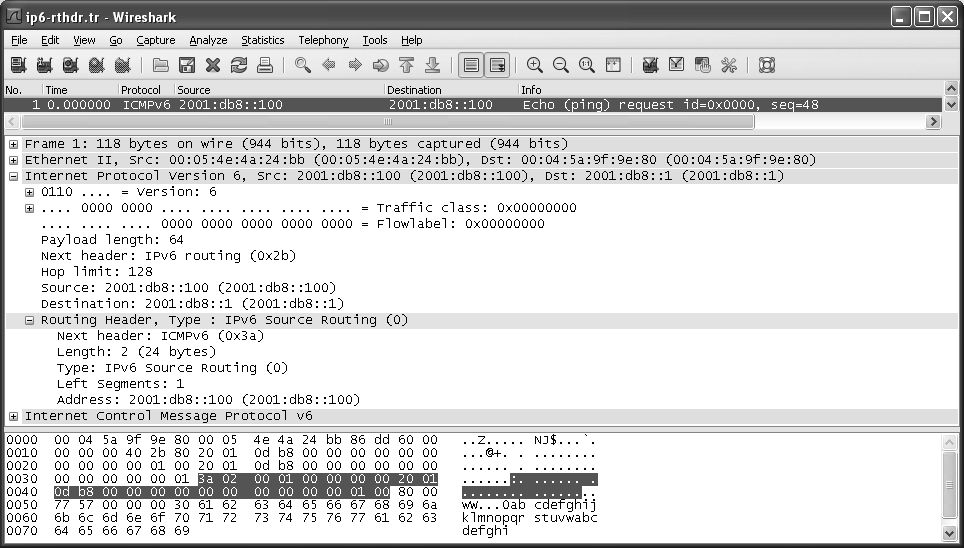
\includegraphics[width=0.7\textwidth]{imgs/5/5-10.png}
  \caption{ping 请求在Wireshark 中显示为一个ICMPv6 回显请求。IPv6 头部包括一个下一个头部字段,
    指出该分组包含一个类型0的路由头部,后面跟着一个 ICMPv6头部。在RHO中需处理的剩
  余网段数 1(2001:db8::100)}
\end{figure}

ping 消息显示为一个ICMPv6 回显请求分组(见第8章)。通过查看下一个头部字段的
值,我们看到在基本头部后面跟着一个路由头部。在路由头部中,我们看到其类型为0(表
示为RHO),还剩余一个网段(跳步)需处理。这个跳步由地址列表(编号0)中的第一个值
指定:2001:db8::100

正如前面提到的,出于安全方面的担心,RHO已在\href{https://www.rfc-editor.org/rfc/rfc5095}{[RFC5095]}中被废弃,因为RHO可
用于增加DoS攻击效果。RHO的问题是允许在路由头部的多个位置指定相同地址。这可能
导致流量在一条特定路径上的两台或多台主机或路由器之间重复转发。大量的流量负载可能
在网络中沿着特定路径创建,与相同路径上的其他流量竞争带宽而造成干扰。因此,RH0目
前已过时,IPv6 唯一支持的路由头部是RH2。RH2与RHO 基本相当,区别在于它只容纳一
个地址,而且在路由类型字段中使用的值不同。

\subsection{分片头部}
分片头部用于IPv6源节点向目的地发送一个大于路径MTU的数据报。对于路径
MTU 以及如何确定它,我们将在第13章中详细讨论,但1280字节是整个网络中针对
IPv6定义的链路层最小MTU(见\href{https://www.rfc-editor.org/rfc/rfc2460}{[RFC2460]}的第5节)。在IPv4
中,如果数据报大小超
过下一跳 MTU,任何主机或路由器可将该数据报分片,IPv4 头部中第二个32位字段表示
分片信息。在IPv6 中,仅数据报的发送者可以执行分片操作,在这种情况下需要添加一个
分片头部。

分片头部包括的信息与IPv4 头部中的相同,只不过标识符字段是32位,而不是IPv4
中采用的16位。这个更大的字段提供了在网络中容纳更多分片的能力。图5-11显示了分片
头部采用的格式。

图5-11

IPv6 分片头部包含一个32位的标识符字段(它是IPv4 中标识符字段的两倍)。M位字段表明
该分片是否为原始数据报的最后一个分片。与IPv4一样,分片偏移字段给出了有效载荷在原
始数据报中以8字节为单位的偏移量

在图5-11中,保留字段和2位的 Res 字段都为0,并且都会被接收方所忽略。分片偏移
字段表明数据以8字节单位的偏移量放置在分片头部之后(相对于原始IPv6数据报的“可
分片部分”,见下一段)。如果 M 位字段设置为1,表示在数据报中包含更多分片。如果该值
为0,表示该分片是原始数据报的最后一个分片。

在分片过程中,输人的数据报称为“原始数据报”,它由两部分组成:“不可分片部分”
和“可分片部分”。不可分片部分包括IPv6 头部和任何在到达目的地之前需由中间节点处
理的扩展头部(即包括路由头部之前的所有头部,如果有逐跳选项扩展头部,则是该头部
之前的所有头部)。可分片部分包括数据报的其余部分(即目的选项头部、上层头部和有效
载荷数据)。

当原始数据报被分片后,将会产生多个分片,其中每个分片都包含一个原始数据报中不
可分片部分的副本,但是需要修改每个IPv6头部的负载长度字段,以反映它所描述的分片
的大小。在不可分片部分之后,每个新的分片都包含一个分片头部,其中包含一个分片相应
的分片偏移字段(例如第一个分片的偏移量0),以及一个原始分组的标识符字段的副本。
最后一个分片的M(更多分片)位字段设置 0。

下面的例子演示了IPv6 源节点对数据报的分片过程。在图5-12所示的例子中,一个
3960字节的有效载荷被分片,其中分片的大小都没有超过1500字节(一个典型的以太网
MTU),分片数据的大小仍为8字节的倍数。

在图5-12 中,我们看到较大的原始数据报被分为3个较小的分片,每个分片都包含一
个分片头部。IPv6头部的负载长度字段被修改,以反映数据和新生成的分片头部的大小。每
个分片中的分片头部包含一个公共标识符字段,以确保网络中不同的原始数据报在其生存期
内不会被分配相同的标识符字段值。

分片头部中的偏移量字段以8字节为单位,因此分片需要在8字节的边界处进行,这
就是第一个和第二个分片包含1448字节,而不是1452字节的原因。因此,除了最后一个分
片之外的所有分片都是8字节的倍数(最后一个分片也可能是)。接收方在对分片进行重组
之前,必须确保已接收原始数据报的所有分片。重组过程需要聚合所有分片以形成原始数据
报。与IPv4 分片一样(见第10章),分片可能不按顺序到达接收方,但需要按顺序重组为一
个数据报,以便交给高层的其他协议处理。

IPv6 分片的例子,1个3960字节的有效载荷被分为3个1448字节或更小的分片。每个分片
包含一个带相同的标识待字段的分片头部。除了最后一个分片,所有分片的更多分片(M)字
段设置为1。偏移量以8字节为单位,例如最后一个分片包含的数据是从原始数据开始处偏
移(362*8)=2896字节。这个方案与IPv4 中的分片相似

在 Windows 7中构造一个 IPv6 分片可使用以下命令:

\begin{verbatim}
    C:> ping -1 3952 ff01::2
\end{verbatim}

图5-13显示了该操作在网络中运行时的 Wireshark 输出。

在图5-13中,我们看到分片由4个发送到IPv6 组播地址 ff01:2 的ICMPv6 回显请求消
息构成。每个请求都需要分片,-13952 选项表示 3952字节的数据携带在每个ICMPv6消息
的数据区中(由于有8字节的ICMPv6头部,因此生成的IPv6负载长度是3960字节)。为了
确定目的地的链路层组播地址,需要执行一个针对IPv6 的特定映射过程,见第9章中的相
关信息。ICMPv6 回显请求(由ping 程序生成)被分散在几个分片中,Wireshark 可显示所有
分片的重组过程。图5-14显示了第二个分片的细节。

在图5-14中,正如预期的那样,我们看到了IPv6头部以及负载长度为1448字节。下
一个头部学段包含一个值44(0x2c),我们通过表5-5可以知道,它表示在IPv6头部之后跟
着一个分片头部。分片头部指出下一个头部为ICMPv6,这意味着没有更多的扩展头部。偏
移量字段181,表示这个分片包含原始数据报中从字节偏移量1448开始的数据。由于
更多分片字段设置为1(在 Wireshark 中显示为 Yes),所以我们知道它不是最后一个分片。
图5-15显示了ICMPv6 回显请求数据报的最后一个分片。

\begin{figure}[!htb]
  \centering
  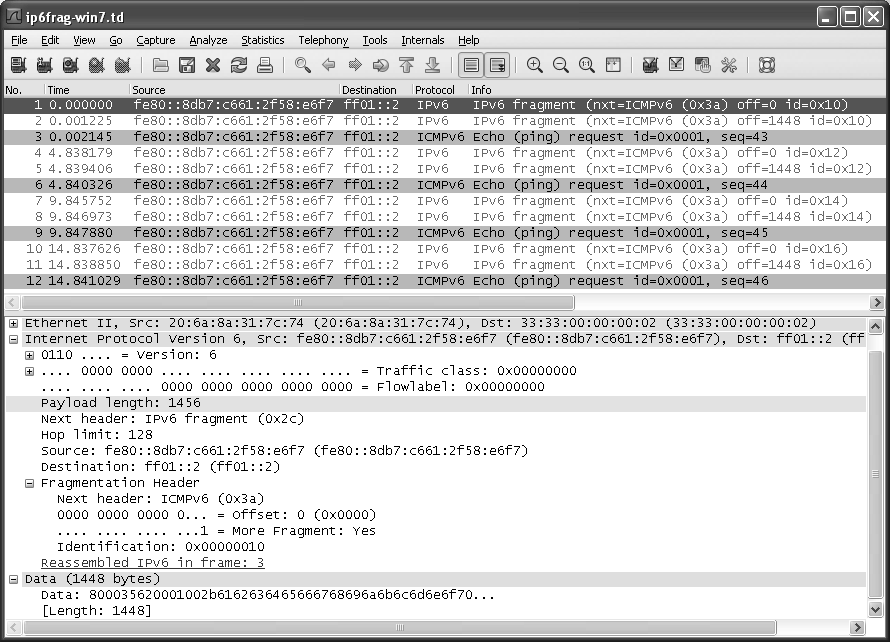
\includegraphics[width=0.7\textwidth]{imgs/5/5-13.png}
  \caption{在这个例子中,ping程序生成了ICMPv6 分组(见第8章),其中包含3960字节的IPV6有
  载荷。这些分组被分成3个分片,每个分片都足够小,以适合以太网的1500字节 MTU 大小}
\end{figure}

\begin{figure}[!htb]
  \centering
  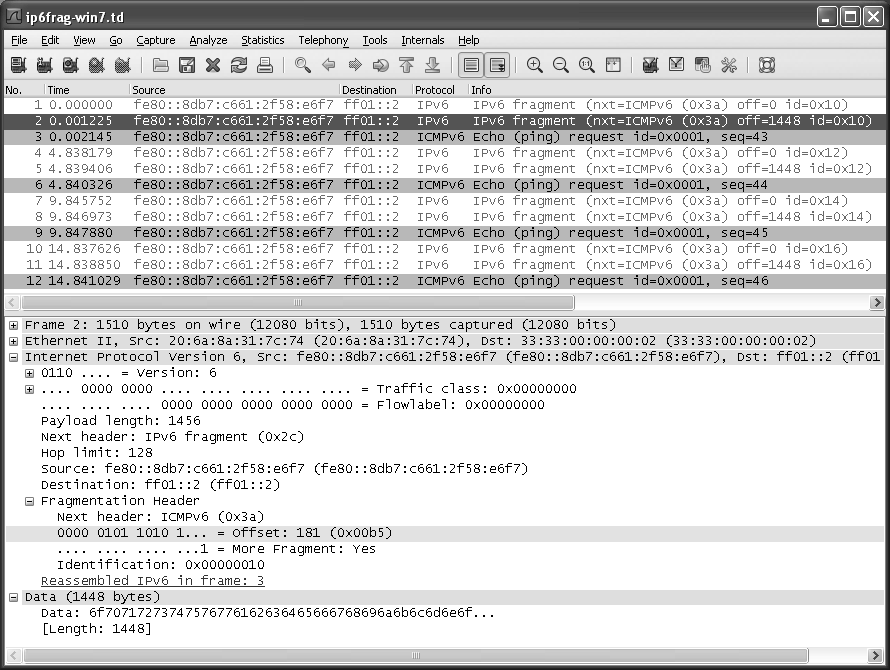
\includegraphics[width=0.7\textwidth]{imgs/5/5-14.png}
  \caption{ICMPv6 回显请求数据报的第二个分片包含1448字节的IPv6 有效载荷,以及8字节的分片
    头部。分片头部表明整个数据报在源节点被分片,偏移量字段的181 表示该分片包含的数扌
    从字节偏移量 1448开始。更多分片(M)位字段被设置,表示需要其他分片共同重组数据报
  同一原始数据报的所有分片包含相同的标识符字段(在这个例子中为2)}
\end{figure}

在图5-15中,我们看到偏移量字段值为362,它是以8字节单位的,也就是说,它相
对于原始数据报的字节偏移量为362*8=2896。总长度字段值为1072,其中包括8字节的分
片头部。Wireshark 为我们计算了分片方式,第一个分片和第二个分片分别包含第一组和第二
组的1448学节,最后一个分片包含1064字节。总的来说,分片过程增加了40*2+8*3=104
字节(2个额外的IPv6头部和每个分片有8字节的分片头部),它们需要由网络层携带。如果
加上链路层的开销,总计104+(2*18)=140字节(每个以太网帧包括一个14字节的头部和
一个4字节的CRC)。

\begin{figure}[!htb]
  \centering
  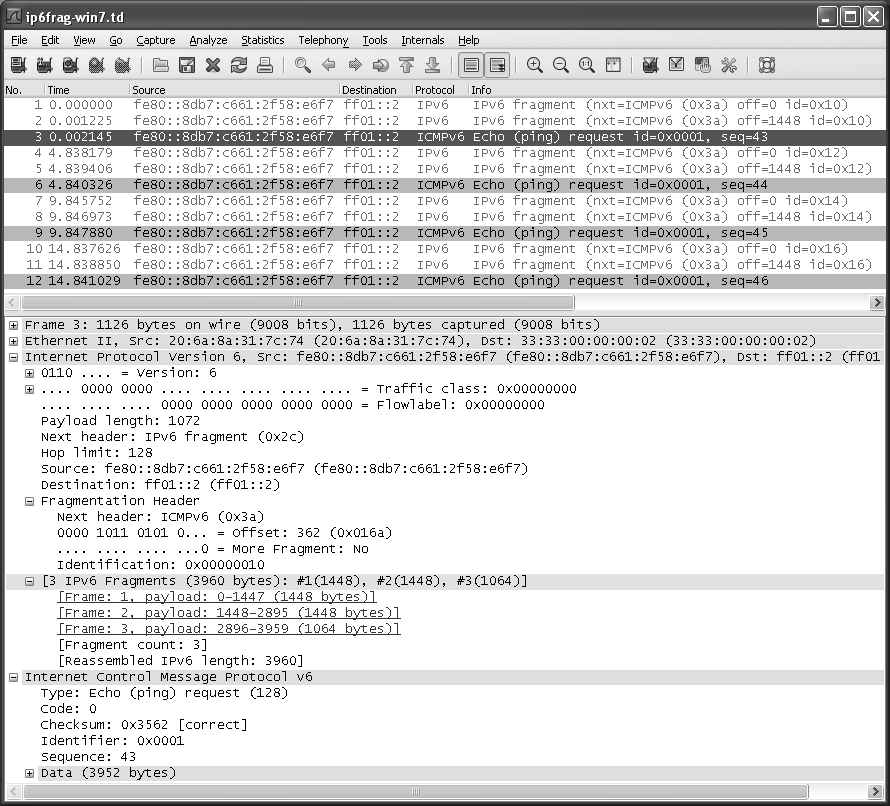
\includegraphics[width=0.7\textwidth]{imgs/5/5-15.png}
  \caption{第一个ICMPv6 回显请求数据报的最后一个分片有 362x8 =2896字节的偏移量和1072字
    节的有效载荷(原始数据报的有效载荷1064字节加上分片头部的8字节)。更多分片字段
    设置为0表示这是最后一个分片,原始数据报的有效载荷总长度为2896+1064 = 3960字节
  (ICMP 数据的3956字节加上ICMPv6头部的8字节;见第8章)}
\end{figure}

\section{IP转发}

从概念上来说,IP转发是很简单的,特别是对于一个主机。如果目的地是直接相连的主
机(例如点到点链接)或共享网络(例如以太网),IP数据报直接发送到目的地,不需要或者
不使用路由器。否则,主机将数据报发送到一台路由器(称为默认路由器),由该路由器将数
据报交付到目的地。这个简单方案适用于大多数主机配置。

在本节中,我们讨论这种简单情况的细节,以及如何在复杂情况下转发IP数据报。首先,
我们注意到当前的大多数主机既可配置为路由器,也可配置为主机,很多家庭网络使用一台连
接到 Internet 的PC作为路由器(也可能是一个防火墙,我们将在第7章中讨论)。主机与路由
器处理 IP 数据报的区别在于:主机不转发那些不是由它生成的数据报,但是路由器会这样做。
在整个方案中,IP协议可接收一个数据报,它可来自同一主机上的其他协议(TCP、UDP
等),也可来自一个网络接口。IP 层包括一些位于内存中的信息,通常称为路由表或转发表,
每次转发一个数据报时需要从中查找信息。当一个网络接口接收到一个数据报时,IP模块首
先检查目的地址是否为自己的IP 地址(与自己的某个网络接口相关的IP 地址),或是它可以
接收其流量的一些其他地址,例如IP广播或组播地址。如果是的话,数据报交付给由IPv4头
部的协议字段或IPv6头部的下一个头部字段指定的协议模块。如果数据报的目的地不是本地
IP模块使用的IP地址,那么:(1)如果IP层配置为一台路由器,则转发该数据报(也就是
说,作为一个输出的数据报处理,见5.4.2 节中的描述);(2)数据报被默默地丢弃。在某些情
况下(例如在情况1中没有路由),ICMP消息可能发送回源节点,以表明发生了一个错误。

\subsection{转发表}
IP 协议标准没有规定转发表所需的精确数据,这个选择工作留给IP 协议的实现者。但
是,IP转发表通常需要包含几个关键信息,我们现在将讨论这些信息。至少在理论上,路由
或转发表中的每个条目包含以下字段信息:

目的地:它是一个32位字段(或128位学段,用于IPv6),用于与一个掩码操作结果
相匹配(见下文)。针对涵盖所有目的地的“默认路由”的情况,目的地可简单地设
零;对于仅描述一个目的地的“主机路由”的情况,目的地可设为完整长度的IP地址。

掩码:它是一个32位字段(或128位字段,用于IPv6),用作数据报目的IP 地址按
位与操作的掩码,其中的目的IP 地址是要在转发表中查找的地址。掩码结果与转发
表条目中的多个目的地进行比较。

下一跳:它是下一个 IP实体(路由器或主机)的32位IPv4地址或128位 IPv6地址,
数据报将被转发到该地址。下一跳实体通常在一个网络中由执行转发查找的系统所共
享,这意味着它们共享同一网络前缀(见第2章)。

接口:它包含一个由IP 层使用的标识符,以确定将数据报发送到下一跳的网络接口。
例如,它可能是一台主机的802.11无线接口、一个有线的以太网接口或一个与串行
端口相关联的PPP接口。如果转发系统也是IP数据报的发送方,该字段用于选择输
出数据报的源IP地址(见5.6.2.1节)。

IP 转发逐跳进行。我们从这个转发表的信息中看到,路由器和主机不包含到任何目的地
的完整转发路径(除了那些直接连接主机或路由器的目的地)。IP 转发只提供数据报发送的
下一跳实体的IP地址。它假设下一跳比执行转发的系统“更接近”目的地,并且下一跳路
由器与执行转发的系统直接连接(即共享同一网络前缀)。它通常也假设与下一跳实体之间没
有“环路”,数据报不会在网络中循环,直至其 TTL 或跳数限制到期。由一个或多个路由协
议来确保路由表正确。多种路由协议能做好这项工作,包括RIP、OSPF、BGP 和 IS-IS,这
里仅列出几种(例如,[DC05] 给出路由协议的更多细节)。

\subsection{IP 转发行动}
当一台主机或路由器中的IP层需要向下一跳的路由器或主机发送一个数据报时,它首
先检查数据报中的目的IP 地址(D)。在转发表中使用该值D来执行最长前缀匹配算法:

1. 在表中搜索具有以下属性的所有条目:\verb|(D^m;)=d|,其中m;是索引为j的转发条目ej
的掩码字段值,d,是转发条目e,的目的地字段值。这意味着目的IP 地址D与每个转发表条
目中的掩码(m,)执行按位与,并将该结果与同一转发条目中的目的地(d)比较。如果满足
这个属性,该条目(这里e)与目的IP 地址相“匹配”。当进行匹配时,该算法查看这个
条目的索引(这里为j),以及在掩码m;中有多少位设置为1。设置为1的位数越多,说明匹
配得“越好”。

2. 选择最匹配的条目ex(即掩码mk 中最多位1 的条目),并将其下一跳字段n作为转
发数据报的下一跳IP地址。

如果在转发表中没有发现匹配的条目,这个数据报无法交付。如果在本地出现(在这台
主机)无法交付的数据报,通常向生成数据报的应用程序返回一个“主机不可达”错误。在
一台路由器上,ICMP消息通常返回给发送数据报的主机。

在某些情况下,可能有多个条目是匹配的(即为1的位数一样)。例如当多个默认路由
可用时会发生这种情况(如连接到多个ISP 时,称为多宿主)。在这种情况下,协议标准没有
规定终端系统的具体行为,而是由具体操作系统的协议实现来决定。通常是简单地选择第一
个匹配的结果。更复杂的系统可能尝试在多个路由上平衡负载或拆分流量。研究表明,多宿
主可能不仅对大型企业有用,也包括家庭用户[THL06]。

\subsection{例子}

为了对简单的局部环境(例如同一LAN)和某些更复杂的多跳环境(全球 Internet)中的
IP 转发工作有深刻的理解,我们将讨论以下两种情况。第一种情况,所有系统使用相同的网
络前缀,这称直接交付;另一种情况为间接交付(见图5-16)。

直接交付不需要路由器,IP数据报封装在一个链路层帧中,它可以直接识别数据来源或目的
地。间接交付涉及路由器,数据转发到这台路由器,并使用该路由器的链路层地址作为目的
地址。路由器的IP 地址没有出现在IP 数据报中(除非路由器自己是源主机或目的主机,或者
使用源路由时)

\subsubsection{直接交付}
我们看一个简单的例子。Windows XP 主机(IPv4 地址S和 MAC地址E) 称为S;一个
IP 数据报发送到Linux 主机(IPv4地址D和MAC地址D),该主机称为D。这些系统通过
一台交换机互连起来。两台主机都在同一以太网中(见封二插图)。图5-16(上)显示了这个
数据报的传输过程。当S的IP 层接收到一个来自上层(例如 TCP 或UDP)的数据报,它将
会查找自己的转发表。我们预期,S的转发表包含的信息如表5-8所示。

表 5-8

主机S中的(单播)IPV4转发表只包含两个条目。主机S配置了IPV4地址和子网掩码
10.0.0.100/25。对于目的地址在10.0.0.1到 10.0.0.126范围内的数据报,使用转发表第二个
条目,并采用直接交付来发送。其他数据报使用第一个条目,并交付给|Pv4 地址为10.0.0.1
的路田器 R
\begin{verbatim}

    目的地

    0.0.0.0

    10.0.0.0

    掩码

    0.0.0.0

    255.255.255.128

    网关(下一跳)

    10.0.0.1

    10.0.0.100

    接

    口

    10.0.0.100

    10.0.0.100
\end{verbatim}

在表5-8中,目的IPv4地址D(10.0.0.9)与第一和第二个转发表条目的匹配。由于它
与第二个条目匹配得更好(25位),所以“网关”或下一跳地址为10.0.0.100,即地址S。该
条目的网关部分包含发送主机的网络接口(没有涉及路由器),说明采用直接交付来发送数
据报。

这个数据报被封装在一个低层帧中,并发送给目的主机D。如果目的主机的低层地址未
知,可能需要使用ARP协议(对于IPv4,见第4章)或邻居请求(对于 IPv6,见第8章)操
作,以确定正确的低层地址D。如果已经知道该地址,数据报中的目的地址是D的IPv4地
址(10.0.0.9),并将D放在低层头部的目的IP地址字段中。这台交换机基于低层地址卫交
付该帧,它并不关心IP地址。

\subsubsection{间接交付}
现在看另一个例子。我们的Windows 主机有一个 IP 数据报发送到主机 ftp.uu.net,其
IPv4地址为192.48.96.9。图5-16(下)显示了通过4台路由器的数据报传输路径(在理论
上)。首先,Windows 主机在自己的转发表中查找,但在本地网络中没有找到匹配的前缀。
这时,它使用自己的默认路由条目(匹配每个目的地,但没有“]”位)。这个默认路由条
目指出适当的下一跳网关为10.0.0.1(路由器R1的“a侧”)。这是一个家庭网络的典型
情况。

我们回想一下直接交付的情况,源IP地址和目的IP地址对应于相应的源主机和目
的主机。对于低层(例如以太网)地址也是这样。在间接交付中,IP地址对应于前面的
源主机和目的主机,但是低层地址不对应。实际上,低层地址决定哪台机器在每跳的基
础上接收包含数据报的帧。在这个例子中,需要的低层地址为下一跳路由器R1的a侧接
口的以太网地址,低层地址对应的IPv4地址为10.0.0.1。这由 ARP(如果在例子中使用
IPv6 则是一个邻居请求),在互联S和R1 的网络上完成。R1通过其a侧的低层地址响应
后,S将向 R1发送数据报。S向R1 交付仅根据低层头部(更具体地说是低层的目的地址)
的处理进行。在接收到这个数据报之后,R1将检查自己的转发表。表5-9中的信息是典
型的。

表5-9 R1的转发表说明需要对流量进行地址转换。路由器一侧是一个私有地址(10.0.0.1),另一侧
是一个公有地址(70.231.132.85)。地址转换用于使来自10.0.0.0/25网络的数据报,看起来
像是从 70.231.132.85 发送到 Internet

\begin{verbatim}
    目的地

    掩

    码

    网关(下一跳)

    0.0.0.0

    0.0.0.0

    70.231.159.254

    10.0.0.0

    255.255.255.128

    10.0.0.100

    接口

    70.231.132.85

    10.0.0.1

    注意

    NAT

    NAT
\end{verbatim}

当R1 接收到数据报时,它发现数据报的目的IP 地址不是自己,因此它将转发这个数据
报。RI搜索转发表,并使用默认的条目。在这种情况下,该默认条目的下一跳位于ISP服
务的网络中,即70.231.159.254(这是R2a侧的接口)。这个地址正好在 SBC的DSL 网络中,
它有一个较长的名称 adsl-70-231-159-254.dsl.snfc21.sbcglobal.net。由于这台路由器位于全球
Internet 中,并且 Windows 机器的源地址为私有地址10.0.0.100,R1对数据报进行网络地址
转换(NAT),以使它在 Internet 中可路由。对数据报进行 NAT处理,结果是生成新的源地址
70.231.132.85,它对应于R1 的b侧接口。不使用私有地址(例如ISP 和大型企业)的网络不
需要执行最后一步,并且保持原来的源地址不变。我们将在第7章中详细介绍 NAT。

当路由器 R2(在ISP 内部)接收到数据报,它的操作步骤与本地路由器R1 相同(除了
NAT操作外)。如果数据报的目的地不是自己的IP 地址,则转发这个数据报。在这种情况
下,路由器通常不仅有一个默认路由,而且有多个其他路由,这取决于它连接的 Internet 的
其他部分,以及它的本地策略。

注意,IPv6转发与传统IPv4 转发只有很少改变。除了更长的地址之外,IPv6还使用一
种稍微不同的机制(邻居请求消息),以确定它的下一跳的低层地址。我们将在第8章中详细
介绍它(作ICMPv6的一部分)。另外,IPv6定义了链路本地地址和全球地址(见第2章)。
全球地址的处理方式就像普通的IP 地址,链路本地地址只能用于同一链路上。另外,所有
的链路本地地址共享相同的IPv6前缀(fe80:/10),在发送一个目的地为链路本地地址的数
据报时,一台多宿主主机可能需要用户来决定使用哪个接口。

为了说明如何使用链路本地地址,我们在自己的 Windows XP 主机上运行(假设IPv6已
启用并且可操作):
\begin{verbatim}
    C:\> ping6 fe80::204:5aff:fe9f:9e80

    Pinging fe80::204:5aff:fe9f:9e80 with 32 bytes of data:

    No route to destination.
        Specify correct scope-id or use -s to specify source address.
        ...

    C:\> ping6 fe80::204:5aff:fe9f:9e80%6

    Pinging fe80::204:5aff:fe9f:9e80%6
    from fe80::205:4eff:fe4a:24bb%6 with 32 bytes of data:

    Reply from fe80::204:5aff:fe9f:9e80%6: bytes=32 time=1ms
    Reply from fe80::204:5aff:fe9f:9e80%6: bytes=32 time=1ms
    Reply from fe80::204:5aff:fe9f:9e80%6: bytes=32 time=1ms
    Reply from fe80::204:5aff:fe9f:9e80%6: bytes=32 time=1ms

    Ping statistics for fe80::204:5aff:fe9f:9e80%6:
        Packets: Sent = 4, Received = 4, Lost = 0 (0% loss),
    Approximate round trip times in milli-seconds:
        Minimum = 1ms, Maximum = 1ms, Average = 1ms
\end{verbatim}

这里,由于没有为链路本地流量指定输出接口,我们将看到一个错误提示。在 Windows
XP 中,我们可指定一个范围ID 或一个源地址。在这个例子中,我们指定的范围ID是一个
使用\%6扩展目的地址的接口号。当发送一个 ping 流量时,通知系统使用接口号6作为正确
的接口。

为了查看一条到达IP 目的地的路径,我们可使用 traceroute 程序(在 Windows 中称次
tracert,它包括的选项稍有不同),使用-n选项表示不将IP 地址转换名称:

\begin{verbatim}
    Linux% traceroute -n ftp.uu.net
    traceroute to ftp.uu.net (192.48.96.9), 30 hops max, 38 byte packets
        1 70.231.159.254 9.285 ms 8.404 ms 8.887 ms
        2 206.171.134.131 8.412 ms 8.764 ms 8.661 ms
        3 216.102.176.226 8.502 ms 8.995 ms 8.644 ms
        4 151.164.190.185 8.705 ms 8.673 ms 9.014 ms
        5 151.164.92.181 9.149 ms 9.057 ms 9.537 ms
        6 151.164.240.134 9.680 ms 10.389 ms 11.003 ms
        7 151.164.41.10 11.605 ms 37.699 ms 11.374 ms
        8 12.122.79.97 13.449 ms 12.804 ms 13.126 ms
        9 12.122.85.134 15.114 ms 15.020 ms 13.654 ms
            MPLS Label=32307 CoS=5 TTL=1 S=0
        10 12.123.12.18 16.011 ms 13.555 ms 13.167 ms
        11 192.205.33.198 15.594 ms 15.497 ms 16.093 ms
        12 152.63.57.102 15.103 ms 14.769 ms 15.128 ms
        13 152.63.34.133 77.501 ms 77.593 ms 76.974 ms
        14 152.63.38.1 77.906 ms 78.101 ms 78.398 ms
        15 207.18.173.162 81.146 ms 81.281 ms 80.918 ms
        16 198.5.240.36 77.988 ms 78.007 ms 77.947 ms
        17 198.5.241.101 81.912 ms 82.231 ms 83.115 ms
\end{verbatim}

这个程序列出了将多个数据报发送到目的地 ftp.uu.net(192.48.96.9)经过的每个IP 跳
步。traceroute 程序使用 UDP数据报(随着时间增大 TTL)和ICMP 消息(用于在UDP数据
报到期时检测每个跳步)共同完成任务。针对每个 TTL 值发送3个UDP分组,以便为每个
跳步测量3次往返时间。在传统上,traceroute 曾经仅携带IP 信息,但在这里我们也看到以
下信息:

\begin{verbatim}
    MPLS Label=32307 CoS=5 TTL=1 S=0
\end{verbatim}

这表明该路径上使用了多协议标签交换(MPLS)\href{https://www.rfc-editor.org/rfc/rfc3031}{[RFC3031]},标签
ID 为32307,服务等级
为5,TTL 为1,并且该消息并不位于
MPLS标签栈底部(S=0;见\href{https://www.rfc-editor.org/rfc/rfc4950}{[RFC4950]})。MPLS是
一种链路层网络,它能够承载多种网络层协议。\href{https://www.rfc-editor.org/rfc/rfc4950}{[RFC4950]}描述了它和ICMP之间的交互,
\href{https://www.rfc-editor.org/rfc/rfc6178}{[RFC6178]}描述了IPv4
分组(包括选项)的处理。很多网络运营商将它用于流量工程(即控
制通过自己网络的流量)。

\subsection{讨论}
在上述例子中,我们应牢记关于IP 单播转发的几个关键点:

\begin{enumerate}
  \item 在这个例子中,大多数主机和路由器使用默认路由,其中包含一个以下形式的转发表
    条目:掩码为0,目的地为0,下一跳为<某些IP 地址>。事实上,在 Internet 边缘,大多
    数主机和路由器会使用一个对所有地址而不是本地网络中的目的地址的默认路由,这是因
    只有一个接口可连接Internet 的其他部分。

  \item 在传统的 Internet 中,数据报中的源IP地址和目的IP地址从不改变。除非是在使用
    源路由的情况下,或沿着传输路径遇到其他功能(例如这个例子中的NAT),否则情况永远
    如此。

  \item 不同的低层头部用于每种链路上的寻址,低层的目的地址(如果存在)总是包含下一
    跳的低层地址。因此,当数据报沿着到目的地的每个跳步移动时,低层头部经常发生变化。
    在我们的例子中,以太网封装的链路层头部中包含下一跳的以太网地址,但是在DSL 链路
    上不会这样做。对于IPv4来说,低层地址通常通过ARP(见第4章)获得;对于IPv6来说,
    则使用ICMPv6 邻居发现(见第8章)。
\end{enumerate}

\section{移动 IP}
到目前为止,我们已讨论了IP数据报通过Internet转发的传统方式,以及使用IP的专
用网络。这个模型的假设是一台主机的IP 地址与附近主机和路由器共享同一前缀。如果这
样一台主机在网络中的连接点改变,但仍保留与链路层网络的连接,它的所有上层(例如
TCP)连接将会失效,这是因它的IP地址必须改变,或路由不能将分组正确交付给(移动
后的)主机。针对它的研究已开展多年(实际上已有几十年),移动IP 解决了这个问题(有人
已提出其他协议,见\href{https://www.rfc-editor.org/rfc/rfc6301}{[RFC6301]})。虽然有各种版本的移动IP—针对IPv4
的\href{https://www.rfc-editor.org/rfc/rfc5944}{[RFC5944]}(称
为MIPv4)和针对IPv6的\href{https://www.rfc-editor.org/rfc/rfc6275}{[RFC6275]},但我们更关注移动IPv6(称
MIPv6),因为它更灵
活和更容易解释。另外,它似乎更容易在快速增长的智能手机上应用。注意,我们不会全面
讨论移动 IPv6,它是非常复杂的,值得专门通过一本书来讨论(例如[RCOS])。但是,我们
将介绍它的基本概念和原则。

移动IP 基于一台主机拥有一个“家乡”网络,但可以不时地访问其他网络的想法。当
主机位于家乡内部时,普通转发基于本章讨论的算法。当主机离开家乡时,它保持平时在家
乡使用的IP 地址,但采用一些特殊的路由和转发手段,使主机可以在这个网络中与其他系
统通信,就好像它仍连接在自己的家乡网络中那样。该方案依赖于一种特殊类型的路由器,
它被称为“家乡代理”,用于为移动节点提供路由。

MIPv6的复杂性主要涉及信令消息,以及如何保证它们的安全。这些消息使用各种形式
的移动扩展头部(表5-5中的下一个头部字段值为135,通常直接称移动头部),因此移动
IP 自身实际上是一种特殊的协议。IANA维护各种头部类型注册信息(目前17被保留),以
及很多与 MIPv6
相关的参数[MP]。我们将关注\href{https://www.rfc-editor.org/rfc/rfc6275}{[RFC6275]}定义的基本信息。其他消息用于
实现“快速切换”\href{https://www.rfc-editor.org/rfc/rfc5568}{[RFC5568]}、改变家乡代理\href{https://www.rfc-editor.org/rfc/rfc5142}{[RFC5142]}和实验目的\href{https://www.rfc-editor.org/rfc/rfc5096}{[RFC5096]}。为了理解
MIPv6,我们开始介绍IP移动的基本模型以及相关术语。

\subsection{基本模型:双向隧道}
图 5-17显示了MIPv6运行中涉及的实体。大部分术语也适用于 MIPv4
\href{https://www.rfc-editor.org/rfc/rfc5944}{[RFC5944]}。一
台可能移动的主机称为移动节点(MN),与它通信的主机称为通信节点(CN)。MN被赋予
一个由家乡网络的网络前缀获得的IP地址。这个地址称为家乡地址(HoA)。当它漫游到一
个可访问的网络时,它被赋予了另一个地址,称为转交地址(CoA)。在基本模型中,当一个
CN 与一个 MN通信时,该流量需要通过MN 的家乡代理(HA)来路由。HA 是一种特殊类
型的路由器,它像其他重要系统(例如路由器和Web 服务器)一样部署在网络基础设施中。
MN 的HOA 和 CoA之间的关联称为 MN 绑定。

图5-17 移动IP 支持节点改变自己的网络连接点,同时保持网络连接操作的能力。移动节点的家乡代
理为移动服务转发流量,并对路由加以优化,通过允许移动,以及在通信节点之间直接通信,
从而极大地提高了路由性能

基本模型(见图5-17)工作在一个 MN的CN不使用 MIPv6 协议的情况下。在整个网
络移动的情况下,这个模型用于支持网络移动(称为“NEMO”
\href{https://www.rfc-editor.org/rfc/rfc3963}{[RFC3963]})。当MN(或
移动网络的路由器)连接到网络中的一个新位置时,它接收自己的CoA,并向自己的HA
发送一个绑定更新消息。这个HA使用一个绑定确认来响应。如果一切顺利,这个MN和
CA 之间的流量通过MN的HA来路由,并使用一种双向的IPv6分组隧道,称双向隧道
\href{https://www.rfc-editor.org/rfc/rfc2473}{[RFC2473]}。这些消息通常使用IPsec
的封装安全有效负载(ESP)来保护(见第18章)。这
样做可确保一个 HA 不会在接收到一个伪造的 MN 绑定更新时被欺骗。

\subsection{路由优化}
双向隧道使MIPv6 工作在一种相对简单的方式下,并使用那些不被移动IP 所感知的
CN,但是路由效率可能非常差,特别是在MN 与CN 之间距离近,但与HA之间距离较远
的情况下。为了改善MIPv6 中可能出现的低效路由,可使用一种称为路由优化(RO)的方
法,只要它被涉及的各个节点支持。正如我们所见,确保 RO安全和可用的方法相当复杂。
我们将描述它的基本操作。更详细的内容见\href{https://www.rfc-editor.org/rfc/rfc6275}{[RFC6275]}和\href{https://www.rfc-editor.org/rfc/rfc4866}{[RFC4866]}。RO
安全相关的设计
原理见\href{https://www.rfc-editor.org/rfc/rfc4225}{[RFC4225]}。

在使用RO时涉及一个通信注册过程,一个MN 将当前CoA通知相应CN,允许它们
执行无须 HA 协助的路由。RO操作分为两部分:一部分涉及注册绑定的建立和维护;另一
部分涉及所有绑定建立后的数据报交换方法。为了与自己的CN建立一个绑定,MN必须向
每个CN证明自己的真实身份。这通过一个返回路由程序(RRP)来完成。支持RRP的消息
在MN 和HA之间不使用IPsec。在MN和CN 之间工作的IPsec 被认为并不可靠(IPv6 需要
IPsec 支持,但不要求必须使用它)。虽然 RRP 不像 IPsec 那样强大,但是它更简单,并涵盖
移动IP设计者关注的大多数安全威胁。

RRP使用以下这些移动消息,它们是IPv6移动扩展头部的子类型:家乡测试初始化
(HoTI)、家乡测试(HOT)、转交测试初始化(CoTI)和转交测试(CoT)。这些消息向CN验
证一个特定 MN的冢乡地址(HoTI 和HoT 消息)和转交地址(CoTI 和CoT 消息)可到达。
这个协议如图5-18 所示。

返回路由检查过程用于从MN 向CN发送绑定更新,以确保路由的优化。该检查的目的是向
CN显示MN 的家乡地址和转交地址都可到达。在本图中,通过间接路由的消息都用虚线箭
头表示。数字表示消息顺序,HOTI 和 CoTI 消息可由MN 同时发送

为了理解RRP,我们来看一个简单例子:只有一个 MN及其HA,以及一个CN,如
图5-18所示。MN开始向CN发送HoTI和CoTI 消息。HoTI消息在到达CN途中通过HA
转发。CN 以某种顺序接收到这两种消息,并分别以HOT和CoT消息响应。HOT消息经由
HA发送到MN。这些消息中包含称为令牌的随机字符串,MIN使用它形成一个加密密钥(见
第18章中对加密和密钥基础知识的讨论)。随后,这个密钥被用于生成发送给CN 的经过
认证的绑定更新。如果成功的话,路由可优化,数据可以在 MN 与CN之间直接传输,如
图5-19所示。

当MN与CN 之间的绑定建立时,数据可以直接在它们之间传输。从MN到CN 的方向使用
IPv6家乡地址目的地选项。相反方向使用类型2的路由头部(RH2)

当一个绑定成功建立后,数据可直接在 MN和CN之间流动,而无须使用效率低的双向
隧道。对于从MN到CN 的流量,可使用IPv6 家乡地址目的地选项;对于相反方向的流量,
可使用类型2的路由头部(RH2),详见图5-19。从MN到CN 的分组中包括MN的CoA的
源 IP
地址字段,从而避免入口过滤问题\href{https://www.rfc-editor.org/rfc/rfc2827}{[RFC2827]},它可能导致包含MN的HOA
的源 IP地
址字段的分组被丢弃。由于包含在家乡地址选项中的MN的HoA 不会被路由器处理,因此
它可不经修改通过路由器到达CN。在返回的路径上,分组被发送到 MN的CoA。在成功接
收返回的分组后,MN处理扩展头部并用包含在RH2中的HoA替换目的IP地址。这个分组
被交付给 MIN 协议栈其余部分,因此应用程序“相信”自己正在使用的是MN的HOA,而
不是用于建立连接和其他操作的 CoA。

\subsection{讨论}
有很多关于移动IP 的问题。它被设计为可处理某种类型的地址移动:一个节点的IP地
址可能改变,同时底层的链路层或多或少保持连接。这种用法对于便携式计算机并不常见,
它们在不同地点之间移动的过程中,通常会关机或进入休眠状态。在需要移动 IP(特别是
MIPv6)的使用模型中,更常见的设备是大量采用IP的智能手机。这些设备可能会运行有
延时要求的实时应用(例如 VoIP)。因此,为了减少执行绑定更新所需的时间,目前已有几
种方法正在探索中。这些方法包括快速切换\href{https://www.rfc-editor.org/rfc/rfc5568}{[RFC5568]}、一种称为分层
MIPv6(HMIPv6)的
MIPv6 修改方案\href{https://www.rfc-editor.org/rfc/rfc5380}{[RFC5380]},以及
MN所需的移动信号由代理执行的修改方案(称代理
MIPv6 或 PMIPv6 \href{https://www.rfc-editor.org/rfc/rfc5213}{[RFC5213]})。

\section{IP 数据报的主机处理}
虽然路由器在转发分组时通常不会考虑将哪个IP 地址放在分组的源IP 地址和目的IP地
址字段中,但主机必须考虑它们。应用程序(例如Web 浏览器)可能尝试连接一台指定的主
机或服务器,它们也可能有多个地址。因此,发送数据报时使用哪个地址(和IP 版本)就有
问题。我们将探讨一个更微妙的事,如果流量到达一个错误的接口(即接收的数据报中存在
未配置的目的地址),是否接收发送到本地IP地址的流量。

\subsection{主机模式}

虽然可能有一个简单的决策方法,确定一个单播数据报是否匹配一台主机的IP地址并
被处理,它取决于接收系统的主机模式\href{https://www.rfc-editor.org/rfc/rfc1122}{[RFC1122]},以及它是否为最相关的多宿主主机。这
里存在两种主机模式:强主机模式和弱主机模式。在强主机模式中,只有当目的IP地址字
段中包含的IP地址与数据报到达的接口配置的IP地址匹配时,才同意把将数据报交付本地
协议栈。在弱主机模式的系统实现中,实际情况相反,一个数据报携带的目的地址与它到达
的任何接口的任何本地地址匹配,无论它到达哪个网络接口,它都会被接收的协议栈处理。
主机模式也适用于发送行为。也就是说,只有当接口配置的地址与发送数据报的源IP地址
字段匹配时,这台采用强主机模式的主机才可从这个特定接口发送数据报。

图5-20显示了一种应用主机模式的情况。在这个例子中,两台主机(A 和B)通过全球
Internet连接,但也可以通过本地网络连接。如果主机A 设置为强主机模式,它从 Internet
接收到一个目的地为203.0.113.1的分组,或从本地网络中接收到一个目的地为192.0.2.1 的
分组,这些分组都会被丢弃。如果主机 B 配置弱主机模式,另一种情况可能会出现。它可
能选择使用本地网络(这样可能更方便或更快)向192.0.2.1 发送分组。不幸的是,当主机 A
接收到某些似乎完全合法的分组,只是由于它运行在强主机模式下,该主机会丢弃这些分
组。因此,我们要提出的一个问题是:为什么强主机模式曾是一个好的方案?

与强主机模式的吸引力相对应的是安全问题。如图5-20所示,恶意用户在 Internet
中生成一个目的地址为203.0.113.2的分组。这个分组可能还包括伪造(“欺骗”)的源IP
地址(例如 203.0.113.1)。如果 Internet 将这个分组路由到主机 B,B 中运行的应用程序可
能被欺骗,相信它接收的流量来源于主机 A。如果应用程序执行基于源IP 地址的访问控制
决策,这样可能带来明显的负面后果。

主机可能通过多个接口连接。在这种情况下,它们必须决定哪些地址用于分组
的源IP地址和目的IP地址字段。这些地址取决于每台主机的转发表、地址选
择算法应用[RFC 3484],以及主机操作使用弱或强主机模式等

无论用于发送还是接收行为,都可在一些操作系统中配置主机模式。在 Windows (Vista
和更高版本)中,强主机模式是IPv4和IPv6发送和接收的默认模式。在 Linux 中,IP操作
默认采用弱主机模式。BSD(包括Mac OS X)使用强主机模式。在Windows 中,以下命令
用于配置基于弱主机的接收和发送行为:

\begin{verbatim}
    C:\> netsh interface ipvx set interface <ifname> weakhostreceive=Yabled

    C:\> netsh interface ipvx set interface <ifname> weakhostsend=Yabled
\end{verbatim}

对于这些命令,<ifname>替换为相应接口名称;X 替换4或6,具体取决于配置的是
哪个版本的IP;而Y替换 en 或 dis,取决于启用还是禁用弱主机模式。

\subsection{地址选择}

当一台主机发送一个 IP数据报时,它必须将自己的IP 地址写人数据报的源IP地址字
段,在它已知多个地址的情况下,数据报的目的地址确定一台特定的目的主机。在有些情况
下源地址是已知的,这是因为它可以由一个应用程序提供,或者为响应同一连接的前一个分
组而发送该分组(详见第13章中如何用 TCP管理地址)。

在当前的IP 实现中,数据报的源IP地址和目的IP 地址字段中使用的IP 地址,是通过
一组称为源地址选择程序和目的地址选择程序获得的。从历史上来看,大多数 Interet 主机
只有一个IP地址用于外部通信,因此选择地址并不是很困难。随着一个接口可使用多个地
址和支持多个地址范围的IPv6的使用,有些程序必须开始使用。当两台实现 IPv4 和 IPv6
(“双协议栈”主机见\href{https://www.rfc-editor.org/rfc/rfc4213}{[RFC4213]})的主机之间通信时,这个情况变得更复杂。地址选择失败
可能导致非对称路由、不必要的过滤或丢弃分组。解决这些问题将是一个挑战。

\href{https://www.rfc-editor.org/rfc/rfc3484}{[RFC3484]}给出了IPv6默认地址的选择规则,纯IPv4
主机通常不会面临这样复杂的问
题。一般情况下,应用程序可调用特定的API执行默认操作,正如上面所提到的那样。即使
这样,棘手的部署问题还是可能出现「RFC52201。「RFC34841中的默认规则是优先在相同范
围内选择成对的源/目的地址,优先选择更小而不是更大的范围以避免在其他地址可用时使
用临时地址,以及优先选择具有更长的通用前缀的成对地址。当全球地址有效时,优先选择
它而不是临时地址。这个规范也包括“管理覆盖”默认规则的方法,但这是具体的部署问题,
我们不做进一步讨论。

默认地址选择通过一个策略表来控制,它(至少在理论上)存在于每台主机中。它是一
个最长匹配前缀查找表,类似于IP 路由使用的转发表。对于一个地址A,在该表中进行一
次查找过程,对A生成一个优先级P(A),以及一个标签L(A)。优先级的数值越大,表示更
加偏好。标签用于相似地址类型的分组。例如,如果L(S) =L(D),该算法倾向于使用该对
(S,D) 作为源/
目的地址对。如果没有规定其他策略,\href{https://www.rfc-editor.org/rfc/rfc3484}{[RFC3484]}建议使用表5-10中的策
略值。

表5-10
\href{https://www.rfc-editor.org/rfc/rfc3484}{[RFC3484]}的默认主机策略表。更高的优先级数值表明一个更大的偏好
\begin{verbatim}

    前缀

    :1/128

    ::/0

    2002::/16

    :/96

    :fh:0:0/96

    优先级 P()

    50

    标签L()

    0

    40

    30

    20

    10

    4
\end{verbatim}

这个表或一个按管理配置参数在站点中配置的表,用于驱动地址选择算法。函数
CPL(A, B) 或“通用前缀长度”,是在IPv6地址A 和B中从最左边的位开始的一个最长通
用前缀的位长度。函数S(A)将IPv6地址A的范围映射到一个数值,范围越大,映射的值越
大。如果A是链路范围,B 是全球范围,则S(A) <S(B)。函数 M(A)将IPv4地址A 映射为
一个IPv4 映射的IPv6地址。由于IPv4地址范围是基于地址自身,因此需要定义以下关系:
S(M(169.254.xx)=S(M(127.xxx)) S(M(专用地址空间))<S(M(任何其他地址))。符号
A(A)是地址的生命周期(见第6章)。如果A是一个过期地址(不鼓励使用的地址),而B是
一个首选地址(优先选择使用的地址),则A(A) < A(B)。最后,如果A是一个家乡地址,则
H(A)为真;如果A是一个转交地址,则C(A)为真。最后两个术语仅用于移动IP 中。

\subsubsection{源地址选择算法}
源地址选择算法定义了一个源地址的候选集合CS(D),它基于一个特定的目的地址
D。这里有一个限制,对于任何D,任播、组播和未指定地址从未出现在CS(D)中。我们
使用符号R(A) 表示地址A在集合CS(D)中的等级。在CS(D)中,A比B的等级更高(即
R(A)值更大),表示R(A)>R(B),意味着优先选择A 而不是B作为到达地址D的源地址。
表达式R(A) *>R(B) 表示在CS(D)中为A分配一个比B更高的等级。符号I(D)表示选
择(通过前面所述的最长匹配前缀转发算法)到达目的地D的接口。符号@(i)是分配给接
口i的地址集合。如果A是一个临时地址(见第6章),T(A)为布尔值true;否则,T(A)为
false。

以下规则用于为目的地D建立地址A和B在CS(D) 中的局部顺序:

\begin{enumerate}
  \item 优先选择相同地址:ifA=D,R(A) *>R(B);ifB=D,R(B) *>R(A)。

  \item 优先选择适当范围:ifS(A) <S(B) and S(A) <S(D),R(B) *>R(A) else R(A)*>R(B);
    if S(B) < S(A) and S(B) <S(D). R(A) *>R(B) else R(B) *>R(A)。

  \item 避免过期地址:ifS(A)=S(B),{if A(A)<A(B),R(B) *>R(A) else R(A) *>R(B)}。

  \item 优先选择家乡地址:if H(A) and C(A) and - (C(B) and H(B)),R(A) *>R(B);if H(B)
    and C(B) and- (C(A) and H(A)),R(B) *> R(A);if (H(A) and - C(A))
    and (-H(B) and C(B)),
    R(A) *> R(B); if (H(B) and - C(B)) and (- H(A) and C(A)),R(B) *>R(A)。

  \item 优先选择输出接口:ifA E @ (I(D)) and B E @ (I(D)),R(A) *R((B); ifB E @ (L((D))
    and A E @ (L(D)),R(B) *>R(A)。

  \item  优先选择匹配标签:if L(A)=L(D) and L(B) L(D),R(A) *>R(B) ;ifL(B)=L(D)
    and L(A) *L(D),R(B) *R(A)。

  \item 优先选择非临时地址:ifT(B) and-T(A),R(A) *> R(B) ;ifT(A) and -T(B),R(B) *>
    R(A)。

  \item 使用最长匹配前缀:if CPL(A, D)> CPL(B, D),R(A) *>R(B);if CPL(B, D)>
    CPL(A, D),R(B) *>R(A)。
\end{enumerate}

局部顺序规则可用于形成CS(D)中所有候选地址的全局顺序。Q(D)表示为目的地D选
择一个最高等级的源地址,它由目的地址选择算法来使用。如果Q(D)=0(空),可能无法为
目的地D确定源地址。

\subsubsection{目的地址选择算法}
我们讨论默认目的地址选择问题。该算法指定了一种类似于源地址选择的方式。回想一

下,Q(D)是上面例子中为目的地D选择的源地址。如果目的地B不可到达,则令 U(B)为布
尔值 true。E(A)表示采用某些“封装传输”(例如,隧道路由)可到达目的地A。集合SD(S)
采用与前面的成对元素 A 和B相同的结构,我们可获得以下规则:

\begin{enumerate}
  \item 避免不可用的目的地:ifU(B) or Q(B)=0,R(A)*>R(B);if U(A) Or Q(A)=0,
    R(B) *>R(A)。

  \item 优先选择匹配范围:ifS(A) =S(Q(A)) and S(B) *S(Q(B)),R(A) *>R(B);if
    S(B) = S(Q(B)) and S(A) *S(Q(A)),R(B) *>R(A).

  \item 避免过期地址:if A(Q(A))<A(Q(B)),R(B)*>R(A);if A(Q(B)) <A(Q(A)),R(A)*>
    R(B)。

  \item 优先选择家乡地址:ifH(Q(A)) and C(Q(A)) and - (C(Q(B)) and H(Q(B))),R(A)*>
    R(B) ; if (Q(B)) and C(Q(B)) and - (C(Q(A)) and H(Q(A))),R(B)
    *>R(A);if (H(Q(A)) and -
    C(O(A))) and (- H(O(B)) and C(Q(B))),R(A) *>R(B); if (H(Q(B)) and
    - C(Q(B))) and (-H(Q(A))
    and C(Q(A))),R(B)*>R(A)。

  \item 优先选择匹配标签:ifL(Q(A))=L(A) and L(Q(B)) *L(B),R(A) *>R(B); ifL(Q(A))*
    L(A) and L(Q(B)) =L(B),R(B)*>R(A)。

  \item 优先选择更高优先级:ifP(A)>P(B),R(A) *>R(B);ifP(A) <P(B), R(B) *>R(A)。

  \item 优先选择本地传输:if E(A) and - E(B),R(B) *>R(A);if E(B) and- E(A),R(A) *
    R(B)。

  \item 优先选择更小范围:ifS(A) <S(B),R(A) *>R(B) else R(B)*> R(A)。

  \item 使用最长匹配前缀:if CPL(A,Q(A))>CPL(B, Q(B)),R(A) *>R(B) ;if CPL(A,
    Q(A)) <CPL(B, Q(B)),R(B) *> R(A)。

  \item 否则,保持等级顺序不变。
\end{enumerate}

针对源地址的选择问题,这些规则形成一个在可能的目的地集合SD(S)中两个元素之
间的偏序。最高等级地址给出了目的地址选择算法的输出。正如前面所说,这个算法操作
(例如目的地址选择的第9步可能导致DNS轮询问题,见第11章)会带来一些问题。因此,
[RFC3484-修订1正考虑对\href{https://www.rfc-editor.org/rfc/rfc3484}{[RFC3484]}加以更新。重要的是,该修订解决了地址选择算法如
何处理唯一本地 IPv6
单播地址(ULA)的问题\href{https://www.rfc-editor.org/rfc/rfc4193}{[RFC4193]}。
ULA是全球范围的IPv6地址,
它被限制只能用于专用网络中。

\section{与IP相关的攻击}

前些年已有一些针对IP 协议的攻击,主要是基于选项操作,或利用专用代码中的错误
(例如分片重组)。由于一个或多个IP 头部字段无效(例如错误的头部长度或版本号),简单
的攻击就能让一台路由器崩溃或性能下降。通常情况下,当前 Internet 中的路由器会忽略或
剥离IP选项,并在基本分组的处理中修复错误。因此,这些类型的简单攻击不是大问题。
涉及分片的攻击可使用其他方法解决\href{https://www.rfc-editor.org/rfc/rfc1858}{[RFC1858]}
\href{https://www.rfc-editor.org/rfc/rfc3128}{[RFC3128]}。

如果没有身份认证或加密(或在IPv6 中被禁用),IP 欺骗攻击是有可能发生的。一些早
期的攻击涉及对源IP地址的伪造。早期的访问控制机制基于源IP地址,很多这样的系统已
不再使用。欺骗有时与源路由选项组合使用。在某些情况下,远程攻击者的计算机可能看起
来像本地网络中的一台主机(甚至是同一计算机)在请求某种服务。虽然IP 地址的欺骗当前
仍然受关注,但有几种方法可限制其危害,包括入口过滤\href{https://www.rfc-editor.org/rfc/rfc2827}{[RFC2827]}\href{https://www.rfc-editor.org/rfc/rfc3704}{[RFC3704]}—ISP
通过
入口过滤检查客户流量的源地址,以确保数据报包含一个指定的IP 前缀。

IPv6 和移动IP 相对较新,至少相对于IPv4来说,它的所有漏洞无疑尚未被发现。由于
有更新、更灵活的选项头部类型,攻击者可对IPv6 分组的处理有相当大的影响。例如,路
由头部(类型0)被发现有严重的安全问题,目前已完全废弃使用它。其他可能的问题包括
源地址和/或路由头部的欺骗,使分组看起来好像来自其他地方。这些攻击可通过配置分组
过滤防火墙,并查看路由头部内容来避免。值得一提的是,如果仅简单地过滤所有包含IPv6
扩展头部和选项的分组,这将会严重限制其使用。特别是,禁用扩展头部将影响移动IPv6
的正常运行。

\section{总结}
在本章中,我们首先介绍IPv4 和IPv6 头部,讨论一些相关的功能,例如 Internet 校验
和与分片。我们分析 IPv6 如何增加地址空间,改进方案包括在分组中使用扩展头部,以及
从IPv4头部中删除一些不重要的字段。随着这些功能的增加,IP 头部大小增大为原来的2
倍,但地址空间增大为原来的4倍。IPv4和IPv6头部不能直接兼容,并且只共享了4位的
版本字段。因此,IPv4和IPv6 节点互连需要某个层次的转换。双协议栈主机需要同时实现
IPv4 和 IPv6,但必须选择何时使用哪种协议。

IP 从出现开始就包含一个头部字段,表示每个数据报的流量类型或服务类别。这种机制
近年来已被重新定义,以便在 Internet 上支持差异化的服务。如果它被广泛实现,Internet 可
能以标准的方式为某些流量或用户提供更好的性能。这种情况能进展到何种程度,部分取决
于围绕差异化服务能力的商业模式的发展。

IP 转发描述了IP 数据报通过单一和多跳网络的传输方式。除了那些需特殊处理的情况,
IP转发在逐跳的基础上进行。数据报的目的IP地址经过每跳时都不改变,但是链路层封装
和链路层目的地址在每跳时会改变。主机和路由器使用转发表和最长前缀匹配算法,以确定
匹配得最好的转发条目,以及沿着一条转发路径的下一跳。在很多情况下,最简单的表只包
含一个默认路由就足够了,只要它能公平匹配所有可能的目的地。

通过一组特殊的安全和信令协议,移动IP在移动节点的家乡地址和转交地址之间建立
安全绑定。这些绑定可用于与移动节点通信,即使它并不在家乡内部。这个基本功能涉及通
过家乡代理的隧道流量,但这可能会导致非常低效的路由。一些额外的功能可支持路由优
化,允许移动节点与其他远程节点直接通信,反之亦然。这要求移动节点的主机支持 MIPv6
和路由优化,它是一个可选的功能。当前研究致力于减少路由优化绑定更新过程中的延时。

我们也讨论了强主机或弱主机模式如何影响IP数据报的处理。在强主机模式下,只允
许每个接口接收或发送包含该接口相关地址的数据报,而弱主机模式的限制较少。弱主机模
式允许在某些特殊情况下通信,但它可能更容易遭受某些形式的攻击。主机模式还涉及主机
如何选择通信时使用的地址。早期,大多数主机只有一个IP地址,因此做出决定相当简单。
一台 IPv6 主机可能有多个IP 地址,多宿主主机可能使用多个网络接口,这时要做出决定并
不容易,并可能对路由产生很大的影响。目前已经有一些地址选择算法(针对源和目的地
址),这些算法倾向于选择范围有限、永久性的地址。

我们讨论了一些针对IP协议的攻击。这种攻击通常涉及地址欺骗,包括利用选项来改
变路由行为,以及试图利用IP 实现中的漏洞,特别是有关分片的漏洞。很多协议实现中的
漏洞在现代操作系统中已修复,在大多数情况下,企业边缘路由器通常会禁用选项。尽管欺
骗仍会受到某些关注,但人口过滤器这类程序有助于解决这个问题。

\section{参考文献}

[A92] P. Mersky, "Autovon: The Dol Phone Company" http://www.chips.navy.
mil/archives/92\_oct/file3.htm

[AN] http://www.iana.org/assignments/protocol-numbers

[DCO5] J. Doyle and J. Carroll, Routing TCP/IP, Volume 1, Second Edition (Cisco
Press, 2005).

[DSCPREG] http://www.iana.org/assignments/dscp-registry/dscp-registry.xml

[H05] G. Huston, "Just How Big Is IPv6?—or Where Did All Those Addresses
Go?" The ISP Column, July 2005, http://cidr-report.org/papers/isoc/2005-07/
ipv6size.html

ILPOPARAM] http://www.iana.org/assignments/ipv6-parameters

[IPPARAM]http://www.iana.org/assignments/ip-parameters

[IV] http://www.iana.org/assignments/version-numbers

[LFS07]J. Leguay, T. Friedman, and K. Salamatian,"Describing and Simulating
Internet Routes" Computer Networks, 51(),June 2007.

[MB97] L. McKnight and J. Bailey, eds., Internet Economics (MIT Press, 1997).

[MP] http://www.iana.org/assignments/mobility-parameters

[P9oJ C. Pinter, A Book of Abstract Algebra, Second Edition (Dover,
2010; reprint of
1990 edition).

[PB61] W. Peterson and D. Brown, "Cyclic Codes for Error Detection" Proc. IRE,
49(228),Jan. 1961.

[RC051 S.Raab and M.Chandra, Mobile IP Technologu and Applications (Cisco
Press, 2005).

[RTAOPTS] http://www.iana.org/assignments/ipv6-routeralert-values

[THL06] N. Thompson, G. He, and H. Luo, "Flow Scheduling for End-Host
homing" Proc. IEEE INFOCOM, Apr. 2006.

[TWEF03] J. Touch, Y. Wang, L. Eggert, and G. Flinn, "A Virtual Internet Ar
tecture"" Proc. ACM SIGCOMM Future Directions in Netwoork Architecture Woi
Mar. 2003.

[W03] T. Wu, "Network Neutrality, Broadband Discrimination"" Journal of T
communications and High Technology Law, 2, 2003 (revised 2005).
